% !TeX root = ../MQF_Manuale_Master.tex
% Capitoli/MQF_Cap_12_Dualita_ALM_Deterministico.tex

\chapter[Dualit\`{a} e ALM deterministico]{Dualit\`{a} e Asset--Liability Management deterministico}

\label{cap:dualita-alm-deterministico}

\medskip

\noindent
\textbf{Obiettivi della lezione.}

Il Capitolo 11 ha introdotto la programmazione lineare attraverso un problema
stilizzato di composizione dell'attivo bancario ispirato al caso Silicon
Valley Bank. La soluzione ottima non \`{e} stata letta soltanto attraverso il
vettore delle decisioni $x^*$ e il valore ottimo $z^*$, ma anche attraverso i
vincoli attivi, l'analisi di sensitivit\`{a} e i valori duali associati ai
diversi requisiti.

Il presente capitolo utilizza questi risultati per compiere un secondo
passaggio. La composizione dell'attivo e della raccolta di una banca non
produce infatti conseguenze soltanto in termini aggregati: attivit\`{a} e
passivit\`{a} generano flussi monetari in date differenti, e una disponibilit\`{a}
di liquidit\`{a} pu\`{o} risultare abbondante in una data e insufficiente in
un'altra. Il problema decisionale deve quindi essere esteso dalla composizione
statica del bilancio al coordinamento intertemporale di attivit\`{a},
passivit\`{a}, liquidit\`{a} e funding.

Al termine del capitolo lo studente dovr\`{a} essere in grado di:

\begin{itemize}

\item utilizzare la relazione tra problema primale e problema duale per
interpretare economicamente il valore marginale dei vincoli;

\item utilizzare dualit\`{a} forte e condizioni di complementariet\`{a} per
collegare soluzione ottima, margini e valori duali;

\item distinguere un requisito aggregato di liquidit\`{a} da un insieme di
fabbisogni distribuiti lungo diverse date;

\item rappresentare mediante una matrice i cash flow prodotti nel tempo dalle
diverse classi di attivo;

\item formulare vincoli di bilancio intertemporali nei quali la liquidit\`{a}
disponibile in un periodo possa essere trasferita al periodo successivo;

\item rappresentare in forma lineare il ricorso a una fonte di funding e il
corrispondente obbligo di rimborso futuro;

\item formulare e interpretare un modello essenziale di
Asset--Liability Management deterministico;

\item interpretare i valori duali dei vincoli temporali come valori marginali
della liquidit\`{a} nelle diverse date;

\item riconoscere quali coefficienti del modello sono trattati come dati
deterministici e comprendere quale modifica concettuale sar\`{a} necessaria
quando tali coefficienti verranno considerati incerti.

\end{itemize}

\section{Dal vincolo aggregato alla struttura temporale del bilancio}

\label{sec:cap12-dal-vincolo-al-tempo}

Il modello sviluppato nel Capitolo~\ref{cap:programmazione-lineare} ha
permesso di isolare alcuni trade-off essenziali nella composizione dell'attivo
bancario. Nel caso SVB stilizzato, le quattro variabili decisionali

\[
x_1,\quad x_2,\quad x_3,\quad x_4
\]

rappresentano rispettivamente cassa e riserve, titoli a breve scadenza, titoli
a lunga scadenza e prestiti o impieghi meno liquidi. La banca sceglie la
composizione che massimizza il risultato economico, rispettando un vincolo di
bilancio, un requisito minimo di liquidit\`a, un limite alla perdita nello
scenario di stress e un limite di concentrazione.

La soluzione numerica ottenuta nel Capitolo 11 \`e

\[
x^*
\approx
\begin{pmatrix}
0\\
41.045\\
20.896\\
38.060
\end{pmatrix},
\qquad
z^*
\approx
3.765.
\]

Il requisito di liquidit\`a \`e

\[
\sum_{j=1}^{4}q_jx_j
\geq
Q_{\min},
\]

e nella soluzione considerata risulta attivo:

\[
\sum_{j=1}^{4}q_jx_j^*
=
Q_{\min}
=
55.
\]

L'analisi di sensitivit\`a e la teoria della dualit\`a sviluppate nel
Capitolo 11 hanno mostrato che a questo requisito pu\`o essere associato un
valore marginale. In prossimit\`a della soluzione considerata, il valore duale
associato al requisito di liquidit\`a \`e

\[
\lambda_Q^*
\approx
0.03507.
\]

La funzione obiettivo misura il risultato economico che la banca cerca di
massimizzare. Un requisito di liquidit\`a pi\`u severo restringe invece
l'insieme delle allocazioni disponibili e pu\`o costringere la banca a
rinunciare a impieghi pi\`u redditizi.

Per questo motivo $\lambda_Q^*$ pu\`o essere interpretato come il
\emph{costo marginale della liquidit\`a}: localmente, un aumento unitario del
requisito $Q_{\min}$ riduce il valore ottimo di circa

\[
0.03507.
\]

Equivalentemente, per una piccola variazione del requisito,

\[
\Delta z^*
\approx
-\lambda_Q^*\,\Delta Q_{\min}.
\]

Il valore duale \`e quindi positivo perch\'e misura il costo marginale della
maggiore prudenza; l'effetto sul risultato massimo \`e negativo perch\'e tale
costo si traduce in una riduzione del risultato economico ottenibile.

Questa lettura completa l'analisi del requisito di liquidit\`a nel modello
statico, ma lascia aperta una questione finanziaria essenziale. Il coefficiente
$q_j$ riassume in un solo numero la capacit\`a dell'attivit\`a $j$ di
contribuire alla liquidit\`a disponibile. Il modello non specifica per\`o
\emph{quando} tale liquidit\`a diventi effettivamente disponibile.

Consideriamo, per esempio, due portafogli che producano cash flow su tre date.
Il portafoglio $A$ genera il profilo

\[
(6,\;2,\;2),
\]

mentre il portafoglio $B$ genera

\[
(1,\;2,\;7).
\]

In entrambi i casi il cash flow complessivo sull'intero orizzonte \`e pari a

\[
10.
\]

Se si considerasse soltanto questa quantit\`a aggregata, i due portafogli
apparirebbero equivalenti sotto il profilo della liquidit\`a.

Supponiamo tuttavia che alla prima data la banca debba fronteggiare un
fabbisogno pari a

\[
d_1=5.
\]

Il portafoglio $A$ produce alla data $t=1$ un cash flow pari a $6$ e pu\`o
quindi soddisfare il fabbisogno. Il portafoglio $B$ produce invece soltanto
$1$: le ulteriori $9$ unit\`a che saranno incassate nelle date successive non
possono essere utilizzate retroattivamente per soddisfare un pagamento che
deve essere effettuato alla prima data.

\begin{figure}[htbp]
\centering
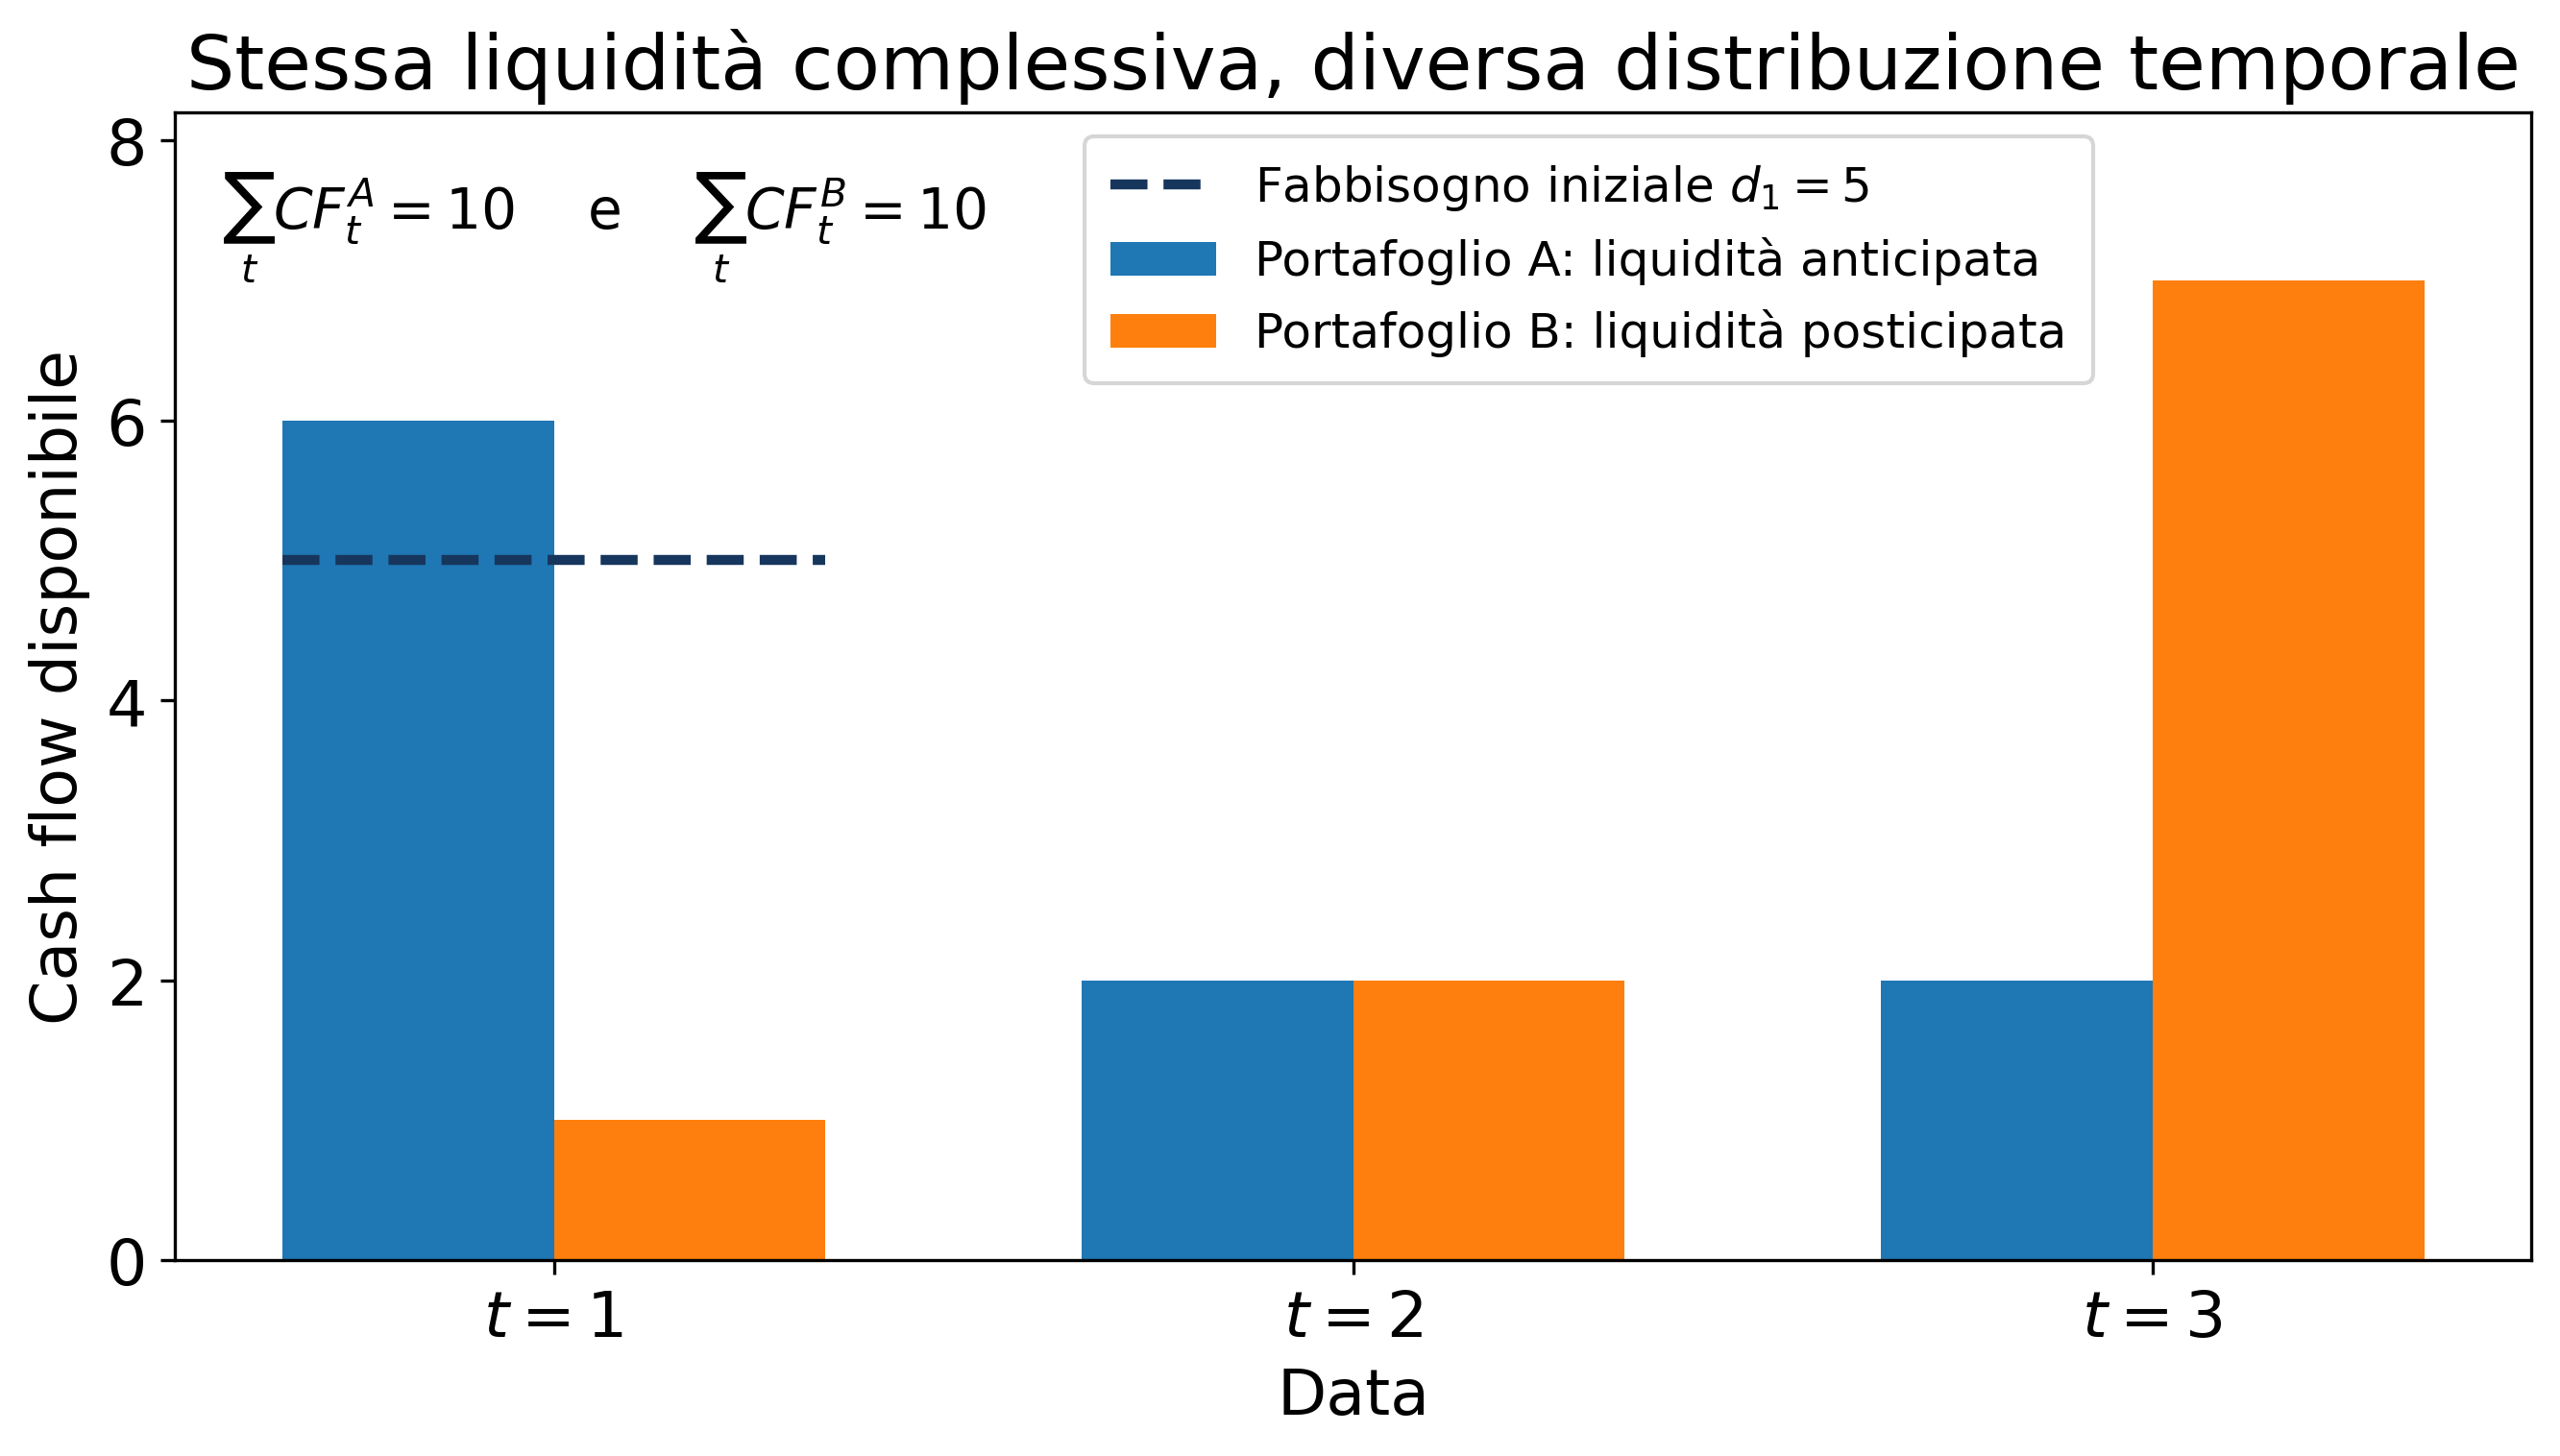
\includegraphics[width=0.90\textwidth]
{../graphics/Cap12_liquidita_aggregata_temporale.png}
\caption{Due portafogli con lo stesso cash flow complessivo ma con diversa
distribuzione temporale. Il portafoglio $A$ produce liquidit\`a in misura
sufficiente a soddisfare il fabbisogno $d_1=5$ alla prima data; il
portafoglio $B$ concentra invece gran parte dei propri flussi alla data
finale.}
\label{fig:cap12-liquidita-aggregata-temporale}
\end{figure}

La Figura~\ref{fig:cap12-liquidita-aggregata-temporale} mostra quindi che la
somma dei cash flow lungo l'intero orizzonte non \`e sufficiente per valutare
la capacit\`a della banca di far fronte ai propri impegni.

La differenza rilevante non riguarda soltanto la quantit\`a complessiva di
liquidit\`a, ma la sua distribuzione nel tempo:

\[
\text{quanto}
\qquad\longrightarrow\qquad
\text{quanto e quando}.
\]

Lo stesso problema si presenta dal lato delle passivit\`a. Una banca non deve
soddisfare un unico fabbisogno aggregato, ma una successione di obblighi,
rimborsi e deflussi collocati in date differenti. La compatibilit\`a tra
attivo e passivo richiede pertanto di confrontare, periodo per periodo, i
flussi prodotti dalle attivit\`a con le risorse richieste dalle passivit\`a.

Introduciamo quindi una sequenza di date

\[
t=0,1,\ldots,T.
\]

Il tempo $t=0$ rappresenta la data nella quale viene scelta la composizione
iniziale del bilancio; le date $t=1,\ldots,T$ rappresentano invece le
scadenze future nelle quali si manifestano cash flow e fabbisogni.

Il problema non consiste pi\`u soltanto nello scegliere una composizione
dell'attivo che soddisfi un requisito complessivo di liquidit\`a. Occorre
scegliere una struttura del bilancio che renda compatibili i flussi generati
dall'attivo con i fabbisogni del passivo lungo l'intero orizzonte temporale.

Il passaggio centrale pu\`o essere sintetizzato come

\[
\boxed{
\text{requisito aggregato di liquidit\`a}
\quad\longrightarrow\quad
\text{bilanci di liquidit\`a alle diverse date}.
}
\]

Questa estensione costituisce il punto di ingresso
nell'Asset--Liability Management deterministico. Il problema resta un
programma lineare: non viene introdotta una nuova classe di ottimizzazione.
Cambiano invece la struttura dei dati e dei vincoli, perch\'e le decisioni
devono ora essere coerenti con una successione di cash flow e fabbisogni
distribuiti nel tempo.

\section{Cash flow degli attivi e fabbisogni alle diverse date}

\label{sec:cap12-cash-flow-fabbisogni}

La sezione precedente ha mostrato che due portafogli con lo stesso cash flow
complessivo possono avere capacit\`a molto diverse di fronteggiare i
fabbisogni della banca. Per rappresentare questa differenza occorre descrivere
separatamente i flussi monetari prodotti alle diverse date.

Consideriamo l'orizzonte discreto

\[
t=0,1,\ldots,T,
\]

e manteniamo il vettore delle decisioni iniziali

\[
x=
\begin{pmatrix}
x_1\\
\vdots\\
x_n
\end{pmatrix},
\]

dove $x_j$ rappresenta l'ammontare destinato alla classe di attivo $j$ al
tempo $0$.

\subsection{Il profilo temporale dei cash flow}

Per ogni attivit\`a $j$ e per ogni data futura $t$, indichiamo con

\[
a_{tj}
\]

il cash flow monetario disponibile alla data $t$ per una unit\`a investita
nell'attivit\`a $j$ al tempo $0$.

L'investimento $x_j$ produce quindi alla data $t$ il flusso

\[
a_{tj}x_j.
\]

Per effetto dell'ipotesi di proporzionalit\`a gi\`a introdotta nel
Capitolo 11, il coefficiente $a_{tj}$ viene trattato come indipendente
dall'ammontare investito. Il cash flow complessivamente prodotto dall'attivo
alla data $t$ \`e pertanto

\[
\sum_{j=1}^{n}a_{tj}x_j.
\]

I coefficienti possono essere raccolti nella matrice dei cash flow

\[
A^{\mathrm{CF}}
=
\begin{pmatrix}
a_{11} & a_{12} & \cdots & a_{1n}\\
a_{21} & a_{22} & \cdots & a_{2n}\\
\vdots & \vdots & \ddots & \vdots\\
a_{T1} & a_{T2} & \cdots & a_{Tn}
\end{pmatrix}.
\]

La matrice $A^{\mathrm{CF}}$ ha $T$ righe e $n$ colonne.

Ogni colonna

\[
\begin{pmatrix}
a_{1j}\\
a_{2j}\\
\vdots\\
a_{Tj}
\end{pmatrix}
\]

descrive il profilo temporale dei cash flow prodotti da una unit\`a della
classe di attivo $j$.

Ogni riga

\[
(a_{t1},\ldots,a_{tn})
\]

descrive invece i cash flow unitari prodotti alla data $t$ dalle diverse
classi di attivo.

Questa organizzazione mantiene la logica matriciale introdotta nel
Capitolo 11. Una colonna continua a descrivere come una variabile decisionale
contribuisce ai diversi requisiti del modello; nel problema multiperiodale,
tali contributi sono ora distinti anche in base alla data nella quale si
manifestano.

\subsection{Il profilo dei fabbisogni}

Dal lato delle passivit\`a, indichiamo con

\[
d_t\geq0
\]

il fabbisogno monetario che deve essere soddisfatto alla data $t$.

La quantit\`a $d_t$ rappresenta l'ammontare di risorse che la banca deve
rendere disponibile in quella data. A seconda della specificazione del
modello, esso pu\`o comprendere rimborsi di passivit\`a, pagamenti
contrattuali, deflussi della raccolta o altri impieghi di liquidit\`a.

Nel modello deterministico sviluppato in questo capitolo, i valori

\[
d_1,d_2,\ldots,d_T
\]

sono trattati come dati noti prima della soluzione del problema e vengono
raccolti nel vettore

\[
d=
\begin{pmatrix}
d_1\\
d_2\\
\vdots\\
d_T
\end{pmatrix}.
\]

La natura deterministica di $d_t$ non implica che i futuri deflussi siano
certi nella realt\`a. Significa che il modello analizza le conseguenze di uno
specifico profilo di fabbisogni assunto come dato nella formulazione
considerata.

Pi\`u avanti il modo in cui tali fabbisogni vengono determinati sar\`a
collegato in modo esplicito alle condizioni economico-finanziarie e alla
situazione patrimoniale della banca. Per il momento, tuttavia, interessa
isolare il problema fondamentale del coordinamento temporale tra risorse
disponibili e risorse richieste.

\begin{figure}[htbp]
\centering
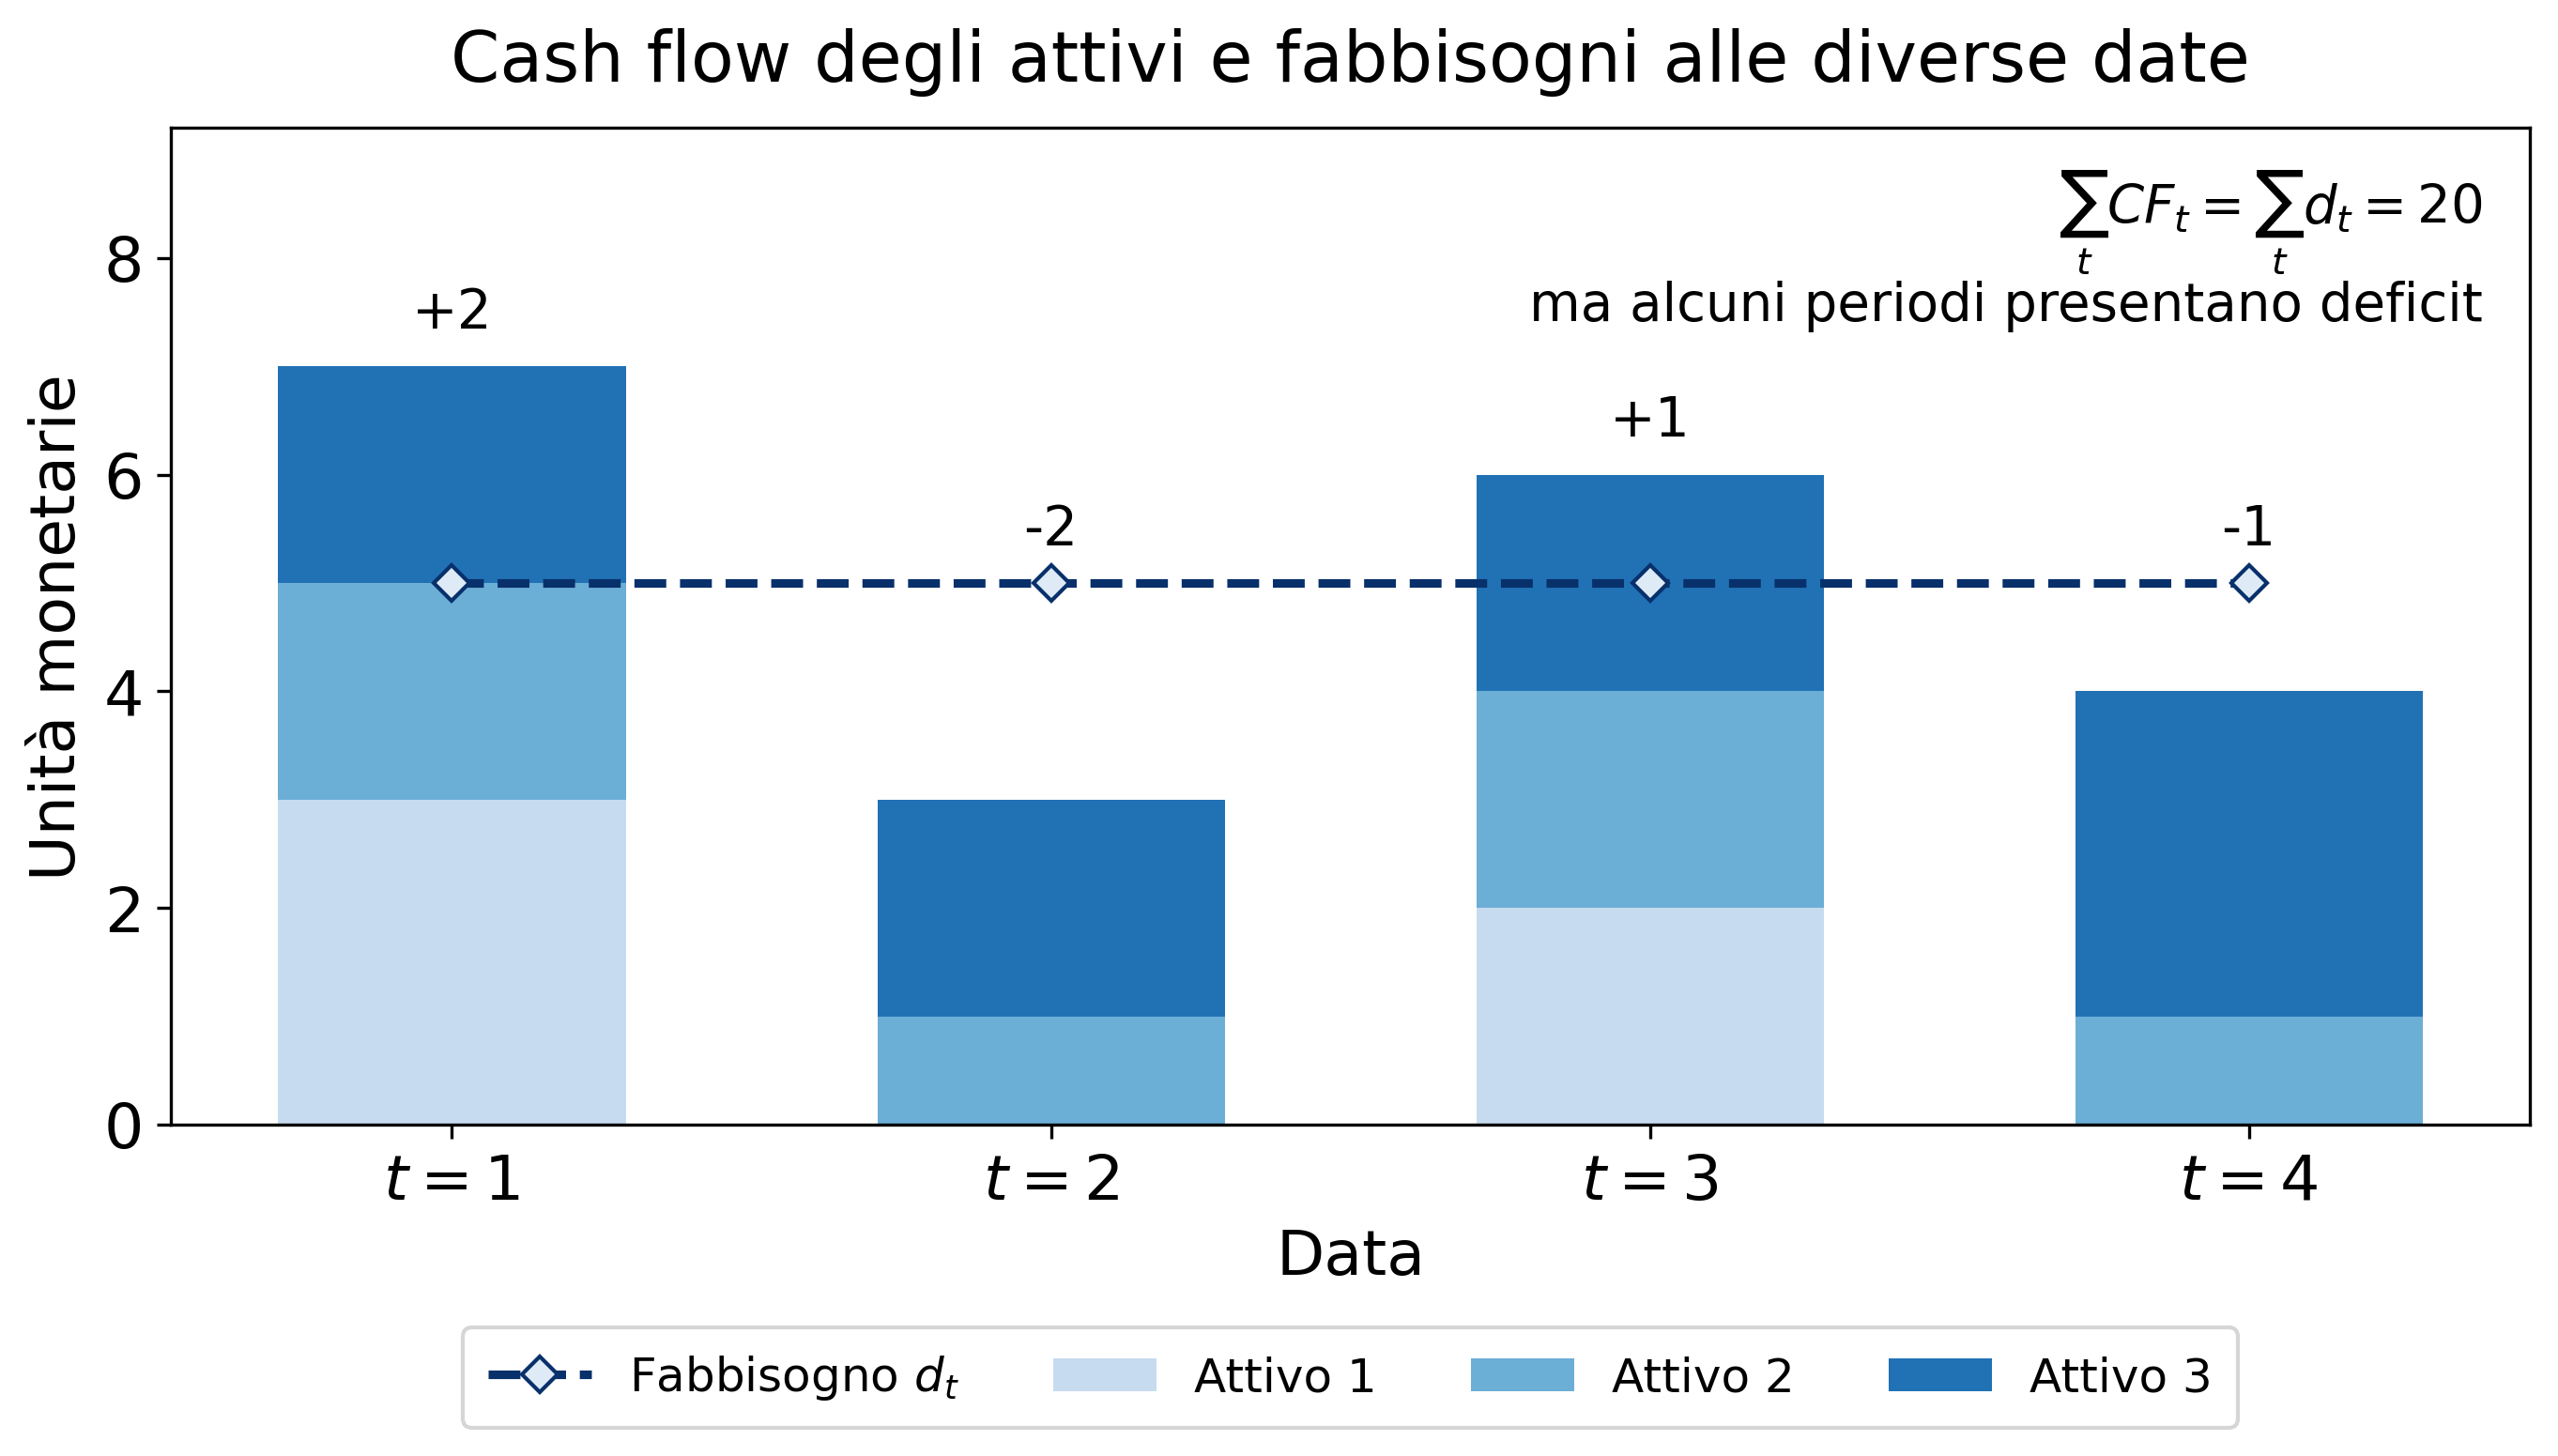
\includegraphics[width=0.92\textwidth]
{../graphics/Cap12_cashflow_attivi_fabbisogni.png}
\caption{Cash flow prodotti dalle diverse classi di attivo e fabbisogni
alle quattro date. Pur coincidendo i cash flow complessivi e i fabbisogni
complessivi sull'intero orizzonte, il profilo temporale presenta surplus
alle date $t=1$ e $t=3$ e deficit alle date $t=2$ e $t=4$.}
\label{fig:cap12-cashflow-fabbisogni}
\end{figure}

La Figura~\ref{fig:cap12-cashflow-fabbisogni} mostra perch\'e il confronto
aggregato non \`e sufficiente. Sull'intero orizzonte le risorse prodotte
dagli attivi coincidono con i fabbisogni:

\[
\sum_{t=1}^{T}CF_t
=
\sum_{t=1}^{T}d_t.
\]

Ci\`o non impedisce tuttavia la presenza di deficit in singole date.
L'Asset--Liability Management deve quindi verificare non soltanto
l'equilibrio complessivo delle risorse, ma la loro disponibilit\`a nel
momento in cui i pagamenti devono essere effettuati.

\subsection{Una prima formulazione: cash-flow matching per data}

Una prima formulazione consiste nel richiedere che, a ciascuna data, i cash
flow prodotti dagli attivi siano almeno sufficienti a coprire il fabbisogno
corrispondente:

\[
\sum_{j=1}^{n}a_{tj}x_j
\geq
d_t,
\qquad
t=1,\ldots,T.
\]

In forma matriciale,

\[
A^{\mathrm{CF}}x
\geq
d.
\]

Il singolo requisito aggregato di liquidit\`a del Capitolo 11 viene quindi
sostituito da $T$ requisiti distinti. La dimensione temporale non viene pi\`u
compressa in un unico coefficiente: per ciascuna data il modello confronta le
risorse monetarie prodotte dall'attivo con il corrispondente fabbisogno.

Questa formulazione rappresenta un primo modello di \emph{cash-flow
matching}. Una composizione dell'attivo \`e ammissibile soltanto se i cash
flow disponibili risultano sufficienti in tutte le date considerate.

Il passaggio dal requisito aggregato

\[
\sum_{j=1}^{n}q_jx_j
\geq
Q_{\min}
\]

ai vincoli

\[
\sum_{j=1}^{n}a_{tj}x_j
\geq
d_t,
\qquad
t=1,\ldots,T,
\]

rende esplicita una differenza fondamentale. Nel primo caso la liquidit\`a
viene misurata come caratteristica complessiva della composizione
dell'attivo; nel secondo viene confrontata con fabbisogni che possiedono una
scadenza precisa.

\subsection{Il limite del matching separato per data}

La formulazione precedente introduce correttamente il tempo, ma considera
ancora ogni data come se fosse indipendente dalle altre.

Supponiamo che, alla data $t$, il portafoglio produca un cash flow superiore
al fabbisogno:

\[
\sum_{j=1}^{n}a_{tj}x_j
>
d_t.
\]

La differenza

\[
\sum_{j=1}^{n}a_{tj}x_j-d_t
\]

rappresenta una disponibilit\`a monetaria residua dopo avere soddisfatto il
fabbisogno della data $t$.

Nei vincoli di cash-flow matching appena formulati, tuttavia, questa
eccedenza non compare nel periodo successivo. Le risorse disponibili alla
data $t$ che non vengono utilizzate scompaiono dal modello e non possono
contribuire alla copertura del fabbisogno alla data $t+1$.

Si tratta di una limitazione economicamente rilevante. Una banca pu\`o
conservare una parte della liquidit\`a disponibile oppure reinvestirla in una
forma compatibile con l'orizzonte successivo. La posizione di liquidit\`a di
una data dipende quindi anche da quanto \`e accaduto nelle date precedenti.

Il problema ALM non pu\`o essere descritto come una semplice successione di
$T$ vincoli indipendenti. Occorre introdurre una variabile che rappresenti la
liquidit\`a residua trasferita da un periodo al successivo.

Il passaggio successivo \`e quindi

\[
\boxed{
\text{cash-flow matching per data}
\quad\longrightarrow\quad
\text{bilanci di liquidit\`a collegati nel tempo}.
}
\]

L'introduzione di questa variabile render\`a esplicita la dipendenza tra il
vincolo relativo alla data $t$ e quello relativo alla data $t+1$ e
costituir\`a il primo vero elemento intertemporale del modello ALM.

\section{Liquidit\`a residua e bilanci intertemporali}

\label{sec:cap12-bilanci-intertemporali}

Il cash-flow matching introdotto nella
Sezione~\ref{sec:cap12-cash-flow-fabbisogni} confronta, per ogni data,
i flussi prodotti dall'attivo con il corrispondente fabbisogno:

\[
\sum_{j=1}^{n}a_{tj}x_j
\geq
d_t,
\qquad
t=1,\ldots,T.
\]

Questa formulazione riconosce che la liquidit\`a deve essere disponibile
nella data in cui viene richiesta, ma non descrive ancora che cosa accade
quando i cash flow prodotti in un periodo superano il fabbisogno dello stesso
periodo.

In una gestione intertemporale, l'eccedenza non scompare. Pu\`o essere
conservata e utilizzata nelle date successive. Per rappresentare questo
meccanismo introduciamo una nuova variabile decisionale.

\begin{definition}[Giacenza di liquidit\`a]

Per ogni data $t=1,\ldots,T$, indichiamo con

\[
g_t\geq0
\]

la liquidit\`a che rimane disponibile immediatamente dopo avere soddisfatto
il fabbisogno $d_t$.

\end{definition}

La variabile $g_t$ \`e quindi uno \emph{stock}, misurato in unit\`a
monetarie. Non rappresenta un nuovo cash flow prodotto dall'attivo, ma la
parte delle risorse disponibili alla data $t$ che non viene utilizzata e
viene trasferita al periodo successivo.

\subsection{Il primo bilancio temporale}

Consideriamo inizialmente la prima data, $t=1$.

I cash flow prodotti dall'attivo sono

\[
\sum_{j=1}^{n}a_{1j}x_j.
\]

Queste risorse devono essere utilizzate per soddisfare il fabbisogno $d_1$;
l'eventuale eccedenza costituisce la giacenza $g_1$.

Il bilancio monetario alla prima data \`e quindi

\[
\sum_{j=1}^{n}a_{1j}x_j
=
d_1+g_1.
\]

La relazione \`e un'uguaglianza, non una disuguaglianza. Tutte le risorse
monetarie disponibili alla data $1$ devono avere una destinazione: una parte
viene utilizzata per soddisfare il fabbisogno, la parte restante viene
conservata come liquidit\`a.

Equivalentemente,

\[
g_1
=
\sum_{j=1}^{n}a_{1j}x_j-d_1.
\]

La condizione

\[
g_1\geq0
\]

garantisce che il fabbisogno della prima data possa essere interamente
soddisfatto.

\subsection{Il collegamento con la data successiva}

Alla data $t=2$ la banca dispone di due fonti di liquidit\`a:

\begin{itemize}

\item i nuovi cash flow prodotti dagli attivi,

\[
\sum_{j=1}^{n}a_{2j}x_j;
\]

\item la giacenza $g_1$ trasferita dalla data precedente.

\end{itemize}

Se, in una prima formulazione, assumiamo che la liquidit\`a trasferita non
produca rendimento, il bilancio alla seconda data diventa

\[
\sum_{j=1}^{n}a_{2j}x_j
+
g_1
=
d_2+g_2.
\]

Pi\`u in generale, per

\[
t=2,\ldots,T,
\]

si ottiene

\[
\sum_{j=1}^{n}a_{tj}x_j
+
g_{t-1}
=
d_t+g_t.
\]

Il sistema completo dei bilanci temporali \`e pertanto

\[
\begin{array}{rcl}
\displaystyle
\sum_{j=1}^{n}a_{1j}x_j
-
g_1
&=&
d_1,
\\[8pt]
\displaystyle
\sum_{j=1}^{n}a_{2j}x_j
+
g_1-g_2
&=&
d_2,
\\
&\vdots&
\\
\displaystyle
\sum_{j=1}^{n}a_{Tj}x_j
+
g_{T-1}-g_T
&=&
d_T.
\end{array}
\]

La differenza rispetto al cash-flow matching separato per data \`e
fondamentale. La variabile $g_t$ compare contemporaneamente nel bilancio
della data $t$ e in quello della data $t+1$.

Il vincolo relativo a una data non pu\`o quindi pi\`u essere interpretato
isolatamente:

\[
\boxed{
g_t
\text{ collega il bilancio della data }t
\text{ al bilancio della data }t+1.
}
\]

Questa \`e la struttura intertemporale essenziale del modello.

\subsection{La liquidit\`a come variabile di stato}

La giacenza $g_t$ possiede una funzione diversa dalle variabili iniziali
$x_j$.

Le quantit\`a

\[
x_1,\ldots,x_n
\]

determinano la composizione dell'attivo \textbf{scelta} al tempo $0$.

La quantit\`a

\[
g_t
\]

descrive invece la posizione di liquidit\`a con la quale la banca conclude la
data $t$ e affronta la data successiva.

In questo senso, $g_t$ pu\`o essere interpretata come una semplice
\emph{variabile di stato}: sintetizza una conseguenza delle decisioni e dei
cash flow passati che diventa rilevante per i vincoli futuri.

Dal bilancio temporale segue infatti la relazione ricorsiva

\[
g_t
=
g_{t-1}
+
\sum_{j=1}^{n}a_{tj}x_j
-
d_t,
\qquad
t=1,\ldots,T,
\]

ponendo per il momento

\[
g_0=0.
\]

La liquidit\`a disponibile alla fine di ogni data dipende quindi dalla
liquidit\`a ereditata dal periodo precedente, dai nuovi flussi prodotti
dall'attivo e dal fabbisogno corrente.

Questa rappresentazione rende esplicito un principio centrale
dell'Asset--Liability Management:

\[
\boxed{
\begin{array}{c}
\text{la posizione finanziaria a una data dipende anche}\\
\text{dalle decisioni e dai saldi accumulati nelle date precedenti}
\end{array}
}
\]

\subsection{Il rendimento della liquidit\`a trasferita}

L'ipotesi secondo cui la liquidit\`a trasferita da una data alla successiva
mantenga invariato il proprio valore \`e utile per isolare la struttura dei
bilanci, ma pu\`o essere raffinata.

Supponiamo che la giacenza disponibile dopo la data $t-1$ possa essere
impiegata fino alla data $t$ a un tasso deterministico $r_{t-1}$.

Una unit\`a monetaria detenuta alla fine della data $t-1$ diventa quindi

\[
1+r_{t-1}
\]

unit\`a alla data $t$.

Per $t=2,\ldots,T$, il bilancio diventa

\[
\sum_{j=1}^{n}a_{tj}x_j
+
(1+r_{t-1})g_{t-1}
=
d_t+g_t.
\]

Per la prima data resta

\[
\sum_{j=1}^{n}a_{1j}x_j
=
d_1+g_1,
\]

se si assume che non esista una giacenza iniziale separata dalla composizione
$x$ scelta al tempo $0$.

Il sistema pu\`o quindi essere scritto come

\[
\begin{array}{rcl}
\displaystyle
\sum_{j=1}^{n}a_{1j}x_j-g_1
&=&
d_1,
\\[8pt]
\displaystyle
\sum_{j=1}^{n}a_{2j}x_j
+
(1+r_1)g_1-g_2
&=&
d_2,
\\
&\vdots&
\\
\displaystyle
\sum_{j=1}^{n}a_{Tj}x_j
+
(1+r_{T-1})g_{T-1}-g_T
&=&
d_T.
\end{array}
\]

Il coefficiente $1+r_{t-1}$ non modifica la natura lineare del modello,
poich\'e il tasso $r_{t-1}$ \`e trattato come un dato deterministico.

\subsection{Condizione finale}

La variabile $g_T$ rappresenta la liquidit\`a residua alla fine
dell'orizzonte considerato. Il suo trattamento dipende dalla funzione del
modello.

Se l'orizzonte termina quando tutti gli obblighi rilevanti sono stati
soddisfatti e non si attribuisce valore alla liquidit\`a residua, pu\`o essere
imposta la condizione

\[
g_T=0.
\]

Se invece la liquidit\`a finale rappresenta una risorsa economicamente utile
oltre l'orizzonte del modello, essa non deve essere forzata a zero: dovr\`a
essere mantenuta come variabile oppure valorizzata nella funzione obiettivo.

La condizione terminale non \`e quindi un dettaglio tecnico. Stabilisce che
cosa il modello considera economicamente rilevante al termine
dell'orizzonte.

\subsection{Dal matching al bilancio dinamico}

Il passaggio compiuto in questa sezione pu\`o essere riassunto confrontando le
due formulazioni.

Nel cash-flow matching separato per data:

\[
\sum_{j=1}^{n}a_{tj}x_j
\geq
d_t.
\]

Nel modello con trasferimento della liquidit\`a:

\[
\sum_{j=1}^{n}a_{tj}x_j
+
(1+r_{t-1})g_{t-1}
=
d_t+g_t.
\]

Nel primo caso ciascuna data costituisce un confronto autonomo tra flussi e
fabbisogni. Nel secondo, il saldo di un periodo diventa una risorsa del
periodo successivo.

La programmazione rimane lineare, ma la struttura economica del problema
cambia profondamente: il modello non confronta pi\`u soltanto attivit\`a e
passivit\`a alle singole date, bens\`i descrive l'evoluzione nel tempo della
posizione di liquidit\`a della banca.

Questo collegamento prepara il passo successivo. La liquidit\`a accumulata
internamente non \`e infatti l'unico strumento con cui una banca pu\`o
fronteggiare un fabbisogno temporaneo. Quando i cash flow dell'attivo e la
giacenza disponibile non sono sufficienti, la banca pu\`o ricorrere a
funding esterno. Tale scelta produce liquidit\`a nella data corrente, ma
genera contemporaneamente un obbligo di rimborso futuro.

\section{Funding esterno e obblighi di rimborso}

\label{sec:cap12-funding}

I bilanci intertemporali introdotti nella
Sezione~\ref{sec:cap12-bilanci-intertemporali} assumono che la banca possa
soddisfare i propri fabbisogni utilizzando esclusivamente i cash flow prodotti
dall'attivo e la liquidit\`a accumulata nelle date precedenti.

Questa rappresentazione mette in evidenza il collegamento temporale tra le
diverse date, ma trascura una possibilit\`a importante. Se le risorse interne
non sono sufficienti a soddisfare un fabbisogno corrente, la banca pu\`o
ricorrere a una fonte esterna di funding.

Il funding modifica la disponibilit\`a di liquidit\`a nella data in cui viene
raccolto, ma non costituisce una risorsa gratuita. Le somme ottenute devono
essere rimborsate in una data successiva insieme al relativo costo
finanziario.

\subsection{Una fonte di funding a un periodo}

Per mantenere leggibile la struttura del modello, consideriamo una sola forma
stilizzata di funding con durata pari a un periodo.

Per

\[
t=1,\ldots,T-1,
\]

indichiamo con

\[
u_t\geq0
\]

l'ammontare di funding raccolto alla data $t$.

La quantit\`a $u_t$ \`e immediatamente disponibile e pu\`o quindi essere
utilizzata per soddisfare il fabbisogno della stessa data.

Supponiamo che il funding raccolto alla data $t$ debba essere rimborsato alla
data $t+1$ a un tasso deterministico $\rho_t$. L'obbligo di rimborso generato
da $u_t$ \`e pertanto

\[
(1+\rho_t)u_t.
\]

La sequenza economica \`e quindi

\[
\boxed{
\begin{array}{c}
\text{funding raccolto alla data }t:\quad u_t\\[3pt]
\downarrow\\[3pt]
\text{liquidit\`a disponibile alla data }t\\[3pt]
\downarrow\\[3pt]
\text{rimborso alla data }t+1:\quad (1+\rho_t)u_t
\end{array}
}
\]

Il funding trasferisce quindi risorse dalla data futura alla data corrente:
aumenta la liquidit\`a disponibile oggi, ma riduce quella disponibile domani.

\subsection{Il bilancio alla prima data}

Alla data $t=1$ la banca dispone dei cash flow prodotti dagli attivi,

\[
\sum_{j=1}^{n}a_{1j}x_j,
\]

e pu\`o inoltre raccogliere funding per un ammontare $u_1$.

Le risorse vengono utilizzate per soddisfare il fabbisogno $d_1$ e
l'eventuale eccedenza viene mantenuta come giacenza $g_1$.

Il bilancio diventa quindi

\[
\sum_{j=1}^{n}a_{1j}x_j
+
u_1
=
d_1+g_1.
\]

Rispetto alla formulazione della sezione precedente, il termine $u_1$
costituisce una nuova fonte di liquidit\`a.

Il suo utilizzo produce tuttavia un effetto sul periodo successivo.

\subsection{Il bilancio nelle date intermedie}

Consideriamo una generica data

\[
t=2,\ldots,T-1.
\]

Le risorse disponibili sono ora costituite da tre componenti:

\begin{itemize}

\item i cash flow prodotti dagli attivi,

\[
\sum_{j=1}^{n}a_{tj}x_j;
\]

\item la giacenza proveniente dalla data precedente, capitalizzata al tasso
$r_{t-1}$,

\[
(1+r_{t-1})g_{t-1};
\]

\item il nuovo funding raccolto alla data corrente,

\[
u_t.
\]

\end{itemize}

A queste risorse si contrappongono tre utilizzi:

\begin{itemize}

\item il fabbisogno corrente $d_t$;

\item il rimborso del funding raccolto alla data precedente,

\[
(1+\rho_{t-1})u_{t-1};
\]

\item la nuova giacenza di liquidit\`a $g_t$.

\end{itemize}

Il bilancio intertemporale completo \`e quindi

\[
\sum_{j=1}^{n}a_{tj}x_j
+
(1+r_{t-1})g_{t-1}
+
u_t
=
d_t
+
(1+\rho_{t-1})u_{t-1}
+
g_t.
\]

La stessa variabile $u_t$ svolge quindi due ruoli in date consecutive:

\[
u_t
\]

\`e una risorsa nel bilancio della data $t$, mentre

\[
(1+\rho_t)u_t
\]

diventa un utilizzo nel bilancio della data $t+1$.

Il funding introduce cos\`i un secondo collegamento intertemporale, accanto a
quello gi\`a prodotto dalla giacenza $g_t$.

\begin{figure}[htbp]
\centering
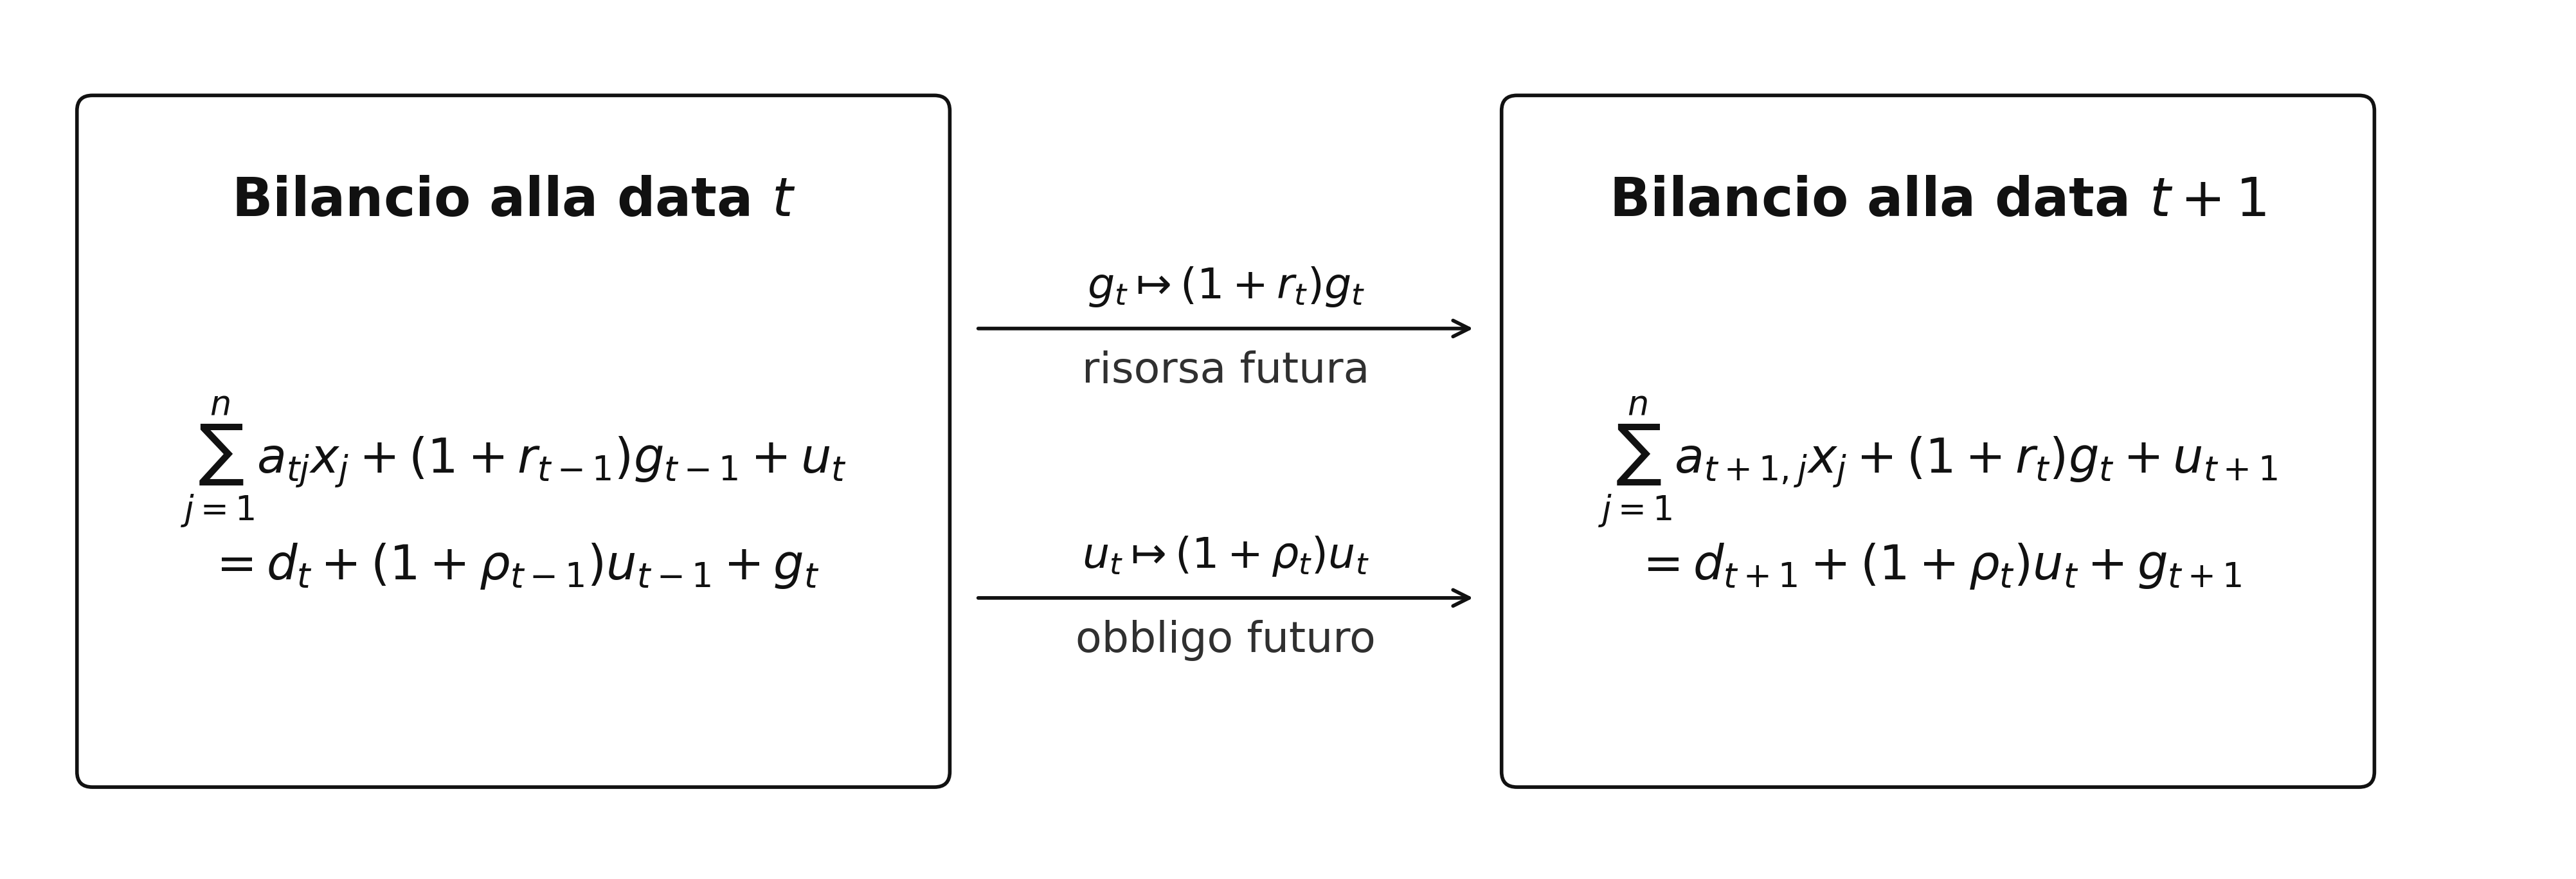
\includegraphics[width=0.96\textwidth]
{../graphics/Cap12_bilancio_intertemporale.png}
\caption{Collegamento tra due bilanci di liquidit\`a consecutivi. La
giacenza $g_t$ costituisce una risorsa disponibile alla data successiva,
mentre il funding $u_t$ raccolto alla data corrente genera un obbligo di
rimborso pari a $(1+\rho_t)u_t$ alla data successiva.}
\label{fig:cap12-bilancio-intertemporale}
\end{figure}

La Figura~\ref{fig:cap12-bilancio-intertemporale} rende visibili i due
collegamenti fondamentali tra date consecutive. La giacenza trasferisce
risorse verso il futuro; il funding trasferisce invece risorse dal futuro
al presente e genera per questo un successivo obbligo di rimborso.

Le due variabili hanno quindi effetti temporali opposti:

\[
g_t
\quad\text{accumula una risorsa per il periodo successivo},
\]

mentre

\[
u_t
\quad\text{anticipa una risorsa creando un'obbligazione futura}.
\]

La struttura intertemporale del modello nasce precisamente dalla presenza
simultanea di questi collegamenti.

\subsection{Il bilancio alla data finale}

Alla data finale $T$ non introduciamo nuovo funding. Questa scelta garantisce
che ogni posizione di funding aperta all'interno dell'orizzonte venga anche
rimborsata entro l'orizzonte stesso.

Il bilancio finale \`e pertanto

\[
\sum_{j=1}^{n}a_{Tj}x_j
+
(1+r_{T-1})g_{T-1}
=
d_T
+
(1+\rho_{T-1})u_{T-1}
+
g_T.
\]

Il sistema completo pu\`o quindi essere scritto come

\[
\begin{array}{rcl}
\displaystyle
\sum_{j=1}^{n}a_{1j}x_j+u_1-g_1
&=&
d_1,
\\[8pt]
\displaystyle
\sum_{j=1}^{n}a_{tj}x_j
+
(1+r_{t-1})g_{t-1}
+
u_t
-
(1+\rho_{t-1})u_{t-1}
-
g_t
&=&
d_t,
\\
&&
t=2,\ldots,T-1,
\\[8pt]
\displaystyle
\sum_{j=1}^{n}a_{Tj}x_j
+
(1+r_{T-1})g_{T-1}
-
(1+\rho_{T-1})u_{T-1}
-
g_T
&=&
d_T.
\end{array}
\]

Le condizioni di non negativit\`a sono

\[
g_t\geq0,
\qquad
t=1,\ldots,T,
\]

e

\[
u_t\geq0,
\qquad
t=1,\ldots,T-1.
\]

\subsection{Limiti alla disponibilit\`a di funding}

La possibilit\`a di raccogliere funding non pu\`o essere considerata
illimitata.

Introduciamo pertanto, per ogni data,

\[
\bar{u}_t\geq0,
\]

che rappresenta l'ammontare massimo di funding accessibile alla banca.

Il vincolo

\[
0\leq u_t\leq\bar{u}_t,
\qquad
t=1,\ldots,T-1,
\]

pu\`o riflettere limiti contrattuali, capacit\`a di accesso al mercato,
disponibilit\`a di linee di credito o altri vincoli sulla raccolta
incrementale.

Il parametro $\bar{u}_t$ ha un significato diverso da $u_t$:

\[
u_t
=
\text{decisione di funding},
\]

mentre

\[
\bar{u}_t
=
\text{massima capacit\`a di funding disponibile}.
\]

La banca decide quindi quanto funding utilizzare all'interno di una
capacit\`a data.

\subsection{Costo del funding e assenza di arbitraggio artificiale}

Il tasso $\rho_t$ rappresenta il costo complessivo della fonte di funding
utilizzata tra le date $t$ e $t+1$.

Nello stesso intervallo, la giacenza di liquidit\`a produce il rendimento
$r_t$.

Per evitare che il modello trovi conveniente raccogliere funding unicamente
per investirlo nella giacenza di liquidit\`a, \`e naturale assumere

\[
\rho_t\geq r_t.
\]

In una rappresentazione bancaria realistica ci si attende normalmente

\[
\rho_t>r_t,
\]

poich\'e la raccolta esterna incorpora un costo superiore al rendimento di una
posizione liquida priva di rischio comparabile.

La differenza

\[
\rho_t-r_t
\]

rappresenta quindi, in forma stilizzata, il costo aggiuntivo associato
all'accesso al funding.

Questa condizione non \`e necessaria per la linearit\`a matematica del
problema, ma evita un comportamento economicamente artificiale del modello.

\subsection{Funding e gestione della liquidit\`a}

L'introduzione di $u_t$ modifica il significato del problema ALM.

Senza funding, un'insufficienza dei cash flow e della liquidit\`a accumulata
rende il piano non ammissibile.

Con il funding, la banca dispone di una seconda possibilit\`a:

\[
\text{deficit corrente}
\quad\longrightarrow\quad
\text{funding oggi}
\quad\longrightarrow\quad
\text{obbligo di rimborso domani}.
\]

Il funding non elimina quindi il problema della liquidit\`a. Ne modifica la
distribuzione temporale.

Una scelta di funding che risolve un deficit alla data $t$ pu\`o infatti
rendere pi\`u difficile soddisfare il bilancio alla data $t+1$, a causa del
rimborso

\[
(1+\rho_t)u_t.
\]

La decisione non pu\`o pertanto essere valutata considerando esclusivamente il
periodo corrente.

Il modello comincia cos\`i a rappresentare il nucleo dell'Asset--Liability
Management:

\[
\boxed{
\begin{array}{c}
\text{le risorse disponibili oggi dipendono dalle decisioni passate,}\\
\text{mentre le decisioni assunte oggi modificano i fabbisogni futuri.}
\end{array}
}
\]

La struttura resta interamente lineare. I coefficienti $a_{tj}$, $d_t$,
$r_t$, $\rho_t$ e $\bar{u}_t$ sono, in questa fase, dati deterministici;
$x_j$, $g_t$ e $u_t$ sono invece le variabili attraverso le quali il modello
descrive la composizione dell'attivo e la gestione intertemporale della
liquidit\`a.

La sezione successiva preciser\`a come tali coefficienti possano essere
ricondotti a un ambiente economico-finanziario deterministico e come il
modello ALM possa essere collegato in modo coerente al caso bancario
sviluppato nel Capitolo 11.

\section{L'ambiente economico-finanziario deterministico}

\label{sec:cap12-ambiente-deterministico}

Le sezioni precedenti hanno costruito la struttura intertemporale del modello
ALM. I cash flow degli attivi, la giacenza di liquidit\`a e il funding
collegano le diverse date attraverso i bilanci

\[
\sum_{j=1}^{n}a_{tj}x_j
+
(1+r_{t-1})g_{t-1}
+
u_t
=
d_t
+
(1+\rho_{t-1})u_{t-1}
+
g_t.
\]

Finora i coefficienti

\[
a_{tj},\qquad r_t,\qquad \rho_t,\qquad \bar{u}_t
\]

sono stati trattati semplicemente come dati del modello. In un problema
bancario, tuttavia, tali coefficienti riflettono le condizioni
economico-finanziarie nelle quali la banca opera.

Per rendere esplicito questo collegamento introduciamo, per ogni data
$t=0,1,\ldots,T$, il vettore

\[
\bar{Z}_t
=
\left(
\bar{R}_t,\bar{C}_t,\bar{F}_t
\right).
\]

La barra indica che, nel presente capitolo, l'intera traiettoria

\[
\bar{Z}_0,\bar{Z}_1,\ldots,\bar{Z}_T
\]

\`e considerata nota al momento della formulazione del problema.

Il modello \`e quindi deterministico, ma i valori dei fattori possono variare
nel tempo:

\[
\bar{Z}_t
\neq
\bar{Z}_{t+1}.
\]

La caratteristica deterministica riguarda la conoscenza della traiettoria,
non la sua costanza.

\subsection{Tre dimensioni dell'ambiente finanziario}

Le tre componenti di $\bar{Z}_t$ hanno funzioni economiche distinte.

Il fattore

\[
\bar{R}_t
\]

rappresenta il livello dei tassi privi di rischio rilevante nell'intervallo
considerato. Esso pu\`o essere interpretato come il \emph{prezzo del tempo}:
determina il rendimento delle disponibilit\`a liquide e contribuisce alla
valutazione dei flussi monetari distribuiti nel tempo.

Il fattore

\[
\bar{C}_t
\]

rappresenta il livello dello spread di credito osservato sul mercato. Esso
misura il premio richiesto per detenere esposizioni soggette a rischio di
credito e pu\`o essere interpretato come il \emph{prezzo del rischio di
credito}.

Il fattore

\[
\bar{F}_t
\]

rappresenta invece lo spread o la tensione associata al funding della banca.
Esso misura quanto l'accesso alla raccolta esterna sia costoso o difficile
rispetto a una fonte priva di rischio comparabile e pu\`o essere interpretato
come il \emph{prezzo della scarsit\`a di funding}.

La distinzione pu\`o essere sintetizzata come

\[
\boxed{
\begin{array}{c}
\bar{R}_t:\ \text{prezzo del tempo},\\[3pt]
\bar{C}_t:\ \text{prezzo del rischio di credito},\\[3pt]
\bar{F}_t:\ \text{prezzo della scarsit\`a di funding}.
\end{array}
}
\]

I tre fattori descrivono l'ambiente esterno nel quale la banca opera. Non
dipendono dalle decisioni $x_j$, $g_t$ o $u_t$ assunte nel modello.

\subsection{Dal livello dei tassi al rendimento della liquidit\`a}

Nella Sezione~\ref{sec:cap12-bilanci-intertemporali} il parametro $r_t$
rappresenta il rendimento ottenibile mantenendo una giacenza di liquidit\`a
tra le date $t$ e $t+1$.

Il suo valore pu\`o essere ricondotto al livello del tasso privo di rischio:

\[
r_t
=
r(\bar{R}_t).
\]

Nella rappresentazione pi\`u semplice, se $\bar{R}_t$ indica direttamente il
tasso applicabile alla giacenza nell'intervallo considerato, si pu\`o porre

\[
r_t=\bar{R}_t.
\]

Il bilancio utilizza quindi

\[
(1+\bar{R}_t)g_t
\]

come ammontare disponibile alla data successiva.

La relazione non deve essere interpretata come una legge generale di mercato.
Essa costituisce una specificazione coerente con un modello nel quale la
liquidit\`a residua viene investita per un periodo in una forma a rischio
trascurabile.

\subsection{Il costo del funding}

Il tasso $\rho_t$ introdotto nella
Sezione~\ref{sec:cap12-funding} rappresenta invece il costo del funding
raccolto alla data $t$ e rimborsato alla data $t+1$.

Il suo valore dipende sia dal livello generale dei tassi sia dalle condizioni
specifiche di funding della banca. Una rappresentazione naturale \`e

\[
\rho_t
=
\rho(\bar{R}_t,\bar{F}_t).
\]

Se $\bar{F}_t$ viene misurato direttamente come spread sul tasso privo di
rischio, una specificazione particolarmente semplice \`e

\[
\rho_t
=
\bar{R}_t+\bar{F}_t.
\]

Il rimborso del funding diventa quindi

\[
\left(
1+\bar{R}_t+\bar{F}_t
\right)u_t.
\]

Questa rappresentazione rende esplicita la differenza tra il rendimento della
liquidit\`a e il costo della raccolta esterna. Se

\[
\bar{F}_t>0,
\]

allora

\[
\rho_t>r_t,
\]

coerentemente con l'ipotesi introdotta nella sezione precedente.

Il funding \`e quindi tanto pi\`u costoso quanto maggiore \`e la tensione
associata alla raccolta della banca.

\subsection{Disponibilit\`a di funding}

Le condizioni di funding possono incidere non soltanto sul costo della
raccolta, ma anche sull'ammontare massimo accessibile.

Il parametro

\[
\bar{u}_t
\]

rappresenta la capacit\`a massima di funding disponibile alla data $t$.

In forma generale si pu\`o scrivere

\[
\bar{u}_t
=
\bar{u}(\bar{F}_t).
\]

In condizioni di funding favorevoli la banca pu\`o disporre di una maggiore
capacit\`a di raccolta; in condizioni di stress tale capacit\`a pu\`o
ridursi.

Non \`e necessario specificare in questa fase una particolare forma
funzionale. Nel problema deterministico, una volta fissata la traiettoria
$\bar{F}_t$, anche

\[
\bar{u}_1,\ldots,\bar{u}_{T-1}
\]

sono coefficienti noti.

Il vincolo

\[
0\leq u_t\leq\bar{u}_t
\]

rimane pertanto lineare.

\subsection{Il ruolo dello spread di credito}

Il fattore $\bar{C}_t$ richiede una precisazione particolare.

Se un'attivit\`a produce cash flow contrattuali certi e viene mantenuta fino
alla scadenza, una variazione dello spread di credito di mercato non modifica
automaticamente tali cash flow.

Non sarebbe quindi corretto introdurre $\bar{C}_t$ nei coefficienti
$a_{tj}$ per il solo fatto che il modello contiene un fattore di credito.

Il fattore $\bar{C}_t$ diventa invece rilevante quando i flussi disponibili
per l'ALM dipendono dalla qualit\`a creditizia o dal valore economico delle
attivit\`a. Ci\`o pu\`o accadere, per esempio, quando il modello considera:

\begin{itemize}

\item cash flow corretti per perdite creditizie;

\item valori di realizzo di titoli o prestiti;

\item haircuts applicati alle attivit\`a utilizzate per ottenere liquidit\`a;

\item valori di mercato di esposizioni creditizie.

\end{itemize}

In tali casi i coefficienti dei cash flow possono essere scritti, in forma
generale, come

\[
a_{tj}
=
a_{tj}
\left(
\bar{R}_t,\bar{C}_t
\right),
\]

per le classi di attivo sensibili a tali fattori.

Per altre attivit\`a, invece, la dipendenza da $\bar{C}_t$ pu\`o essere
assente.

Questa distinzione \`e importante: non tutti i fattori economici devono
entrare in tutti i coefficienti del modello.

\subsection{Fattori esterni e coefficienti del modello}

La relazione tra ambiente esterno e parametri ALM pu\`o essere sintetizzata
come

\[
\bar{Z}_t
=
(\bar{R}_t,\bar{C}_t,\bar{F}_t)
\quad\longrightarrow\quad
\left\{
a_{tj},\,
r_t,\,
\rho_t,\,
\bar{u}_t
\right\}.
\]

Il vettore $\bar{Z}_t$ descrive condizioni economico-finanziarie esterne.

I coefficienti

\[
a_{tj},\qquad r_t,\qquad \rho_t,\qquad \bar{u}_t
\]

traducono tali condizioni nella struttura quantitativa del problema ALM.

Una volta fissata la traiettoria

\[
\bar{Z}_0,\ldots,\bar{Z}_T,
\]

tutti questi coefficienti sono numeri noti. Il problema rimane quindi un
programma lineare deterministico.

In particolare, la dipendenza dei coefficienti dall'ambiente esterno non
introduce non linearit\`a nelle variabili decisionali, poich\'e

\[
\bar{Z}_t
\]

non costituisce una variabile scelta dalla banca.

\subsection{Ci\`o che l'ambiente esterno non descrive}

Il vettore $\bar{Z}_t$ non contiene informazioni sulla solidit\`a interna
della banca.

Due banche possono trovarsi, alla stessa data, nelle medesime condizioni di
tassi, spread creditizi e funding:

\[
\bar{Z}_t^{(A)}
=
\bar{Z}_t^{(B)},
\]

ma avere strutture patrimoniali molto differenti.

Una banca pu\`o disporre di abbondante liquidit\`a, perdite contenute e
capitale elevato; un'altra pu\`o presentare forte esposizione a perdite di
mercato, liquidit\`a limitata e una struttura di funding pi\`u fragile.

Tali differenze non devono essere incorporate artificialmente nel vettore
$\bar{Z}_t$. Esse dipendono dallo stato della banca, che \`e a sua volta il
risultato delle decisioni assunte e dei flussi accumulati nel tempo.

Occorre pertanto distinguere due livelli:

\[
\boxed{
\begin{array}{c}
\bar{Z}_t:
\text{ condizioni economico-finanziarie esterne},\\[4pt]
X_t:
\text{ stato patrimoniale e finanziario della banca}.
\end{array}
}
\]

Il primo \`e esogeno rispetto alle decisioni della banca; il secondo evolve
anche come conseguenza delle decisioni precedenti.

La sezione successiva introdurr\`a questa distinzione in modo esplicito e
mostrer\`a come lo stato della banca e l'ambiente esterno concorrano a
determinare la sua solidit\`a e i fabbisogni di liquidit\`a.

\section{Stato della banca, solidit\`a e fabbisogni di liquidit\`a}

\label{sec:cap12-stato-banca}

La Sezione~\ref{sec:cap12-ambiente-deterministico} ha descritto le condizioni
economico-finanziarie esterne attraverso il vettore

\[
\bar Z_t
=
(\bar R_t,\bar C_t,\bar F_t).
\]

Questi fattori incidono sui tassi, sul valore delle attivit\`a e sulle
condizioni di accesso al funding. Essi non descrivono tuttavia la situazione
interna della banca.

A parit\`a di condizioni di mercato, due banche possono presentare capacit\`a
molto diverse di assorbire uno shock di liquidit\`a. Una banca pu\`o disporre
di abbondanti attivit\`a liquide, capitale elevato e limitata dipendenza dal
funding; un'altra pu\`o trovarsi nella situazione opposta.

Per distinguere questi due livelli introduciamo lo stato interno della banca.

\begin{definition}[Stato della banca]

Indichiamo con

\[
X_t
\]

il vettore che descrive le variabili patrimoniali e finanziarie della banca
rilevanti alla data $t$.

\end{definition}

Le componenti precise di $X_t$ dipendono dal livello di dettaglio del modello.
Possono comprendere, per esempio:

\begin{itemize}

\item la composizione e il valore delle attivit\`a;

\item la disponibilit\`a di liquidit\`a;

\item la consistenza del capitale;

\item le passivit\`a in essere;

\item il funding precedentemente raccolto e ancora da rimborsare.

\end{itemize}

Nel modello costruito nelle sezioni precedenti, la giacenza $g_t$ e gli
obblighi generati dal funding sono quindi esempi di informazioni che
contribuiscono a determinare lo stato della banca.

\subsection{Ambiente esterno e stato interno}

La distinzione tra $\bar Z_t$ e $X_t$ \`e essenziale.

Il vettore

\[
\bar Z_t
\]

descrive condizioni che la singola banca considera esterne alle proprie
decisioni.

Il vettore

\[
X_t
\]

descrive invece la posizione con la quale la banca affronta quelle
condizioni.

Possiamo quindi rappresentare schematicamente la situazione alla data $t$
come

\[
(\bar Z_t,X_t).
\]

Due banche possono affrontare lo stesso ambiente,

\[
\bar Z_t^{(A)}
=
\bar Z_t^{(B)},
\]

ma avere stati interni differenti,

\[
X_t^{(A)}
\neq
X_t^{(B)}.
\]

Esse possono pertanto reagire in modo molto diverso allo stesso shock.

Questa distinzione evita di attribuire all'ambiente di mercato caratteristiche
che appartengono invece al bilancio della singola banca.

\subsection{Un indicatore di solidit\`a}

Per sintetizzare la capacit\`a della banca di fronteggiare le condizioni
economico-finanziarie correnti introduciamo un indicatore di solidit\`a o
resilienza

\[
h_t.
\]

In forma generale possiamo scrivere

\[
h_t
=
h(X_t,\bar Z_t).
\]

L'indicatore dipende quindi sia dallo stato interno della banca sia
dall'ambiente nel quale tale stato deve essere valutato.

Lo stesso livello di liquidit\`a o di capitale pu\`o infatti assumere un
significato diverso in condizioni di mercato normali o in presenza di forte
tensione sul funding e sugli spread.

Non \`e necessario, in questa fase, specificare una particolare funzione
$h(\cdot)$. Ci interessa soprattutto distinguere le determinanti della
solidit\`a:

\[
\boxed{
\begin{array}{c}
\text{solidit\`a della banca}\\[3pt]
\uparrow\\[3pt]
\text{stato interno }X_t
\quad+\quad
\text{ambiente esterno }\bar Z_t.
\end{array}
}
\]

L'indicatore $h_t$ non rappresenta quindi un nuovo fattore di mercato. \`E
una caratteristica della banca valutata nelle condizioni di mercato
correnti.

\subsection{Dalla solidit\`a ai deflussi}

La relazione tra stato della banca e liquidit\`a diventa particolarmente
importante quando si considerano i deflussi della raccolta.

In una rappresentazione pi\`u ricca, il fabbisogno di liquidit\`a alla data
$t$ non dipenderebbe necessariamente soltanto dall'ambiente esterno.
Potrebbe dipendere anche dalla solidit\`a percepita della banca.

In termini schematici si potrebbe scrivere

\[
d_t
=
d(\bar Z_t,h_t),
\]

e quindi

\[
d_t
=
d\left(
\bar Z_t,
h(X_t,\bar Z_t)
\right).
\]

La struttura esprime un meccanismo economicamente importante:

\[
\bar Z_t
\longrightarrow
h_t
\longrightarrow
d_t,
\]

ma anche

\[
X_t
\longrightarrow
h_t
\longrightarrow
d_t.
\]

Uno shock esterno pu\`o quindi generare conseguenze diverse a seconda della
condizione patrimoniale con cui la banca lo affronta.

Per esempio, una tensione generalizzata sul funding pu\`o risultare
gestibile per una banca con ampia disponibilit\`a di attivit\`a liquide e
capitale elevato, mentre pu\`o produrre un fabbisogno molto pi\`u severo per
una banca con struttura finanziaria fragile.

\subsection{La retroazione delle decisioni sullo stato della banca}

Lo stato interno non rimane necessariamente invariato nel tempo.

Le decisioni prese alla data $t$ modificano infatti la posizione con la quale
la banca affronta la data successiva.

In forma generale possiamo rappresentare questa evoluzione come

\[
X_{t+1}
=
G(X_t,u_t,\bar Z_t,d_t),
\]

dove la funzione $G(\cdot)$ sintetizza le relazioni contabili e finanziarie
che determinano il nuovo stato.

Il funding $u_t$, per esempio, aumenta le risorse disponibili alla data $t$,
ma genera un obbligo di rimborso futuro. Analogamente, la liquidit\`a
residua $g_t$ migliora la posizione con la quale la banca affronta il periodo
successivo.

La sequenza concettuale diventa quindi

\[
\boxed{
\begin{array}{ccccc}
\bar Z_t
&
\longrightarrow
&
h_t,\ d_t
&
\longrightarrow
&
u_t
\\[3pt]
&&
\uparrow
&&
\downarrow
\\[-2pt]
&&
X_t
&&
X_{t+1}.
\end{array}
}
\]

L'ambiente esterno influenza le condizioni nelle quali la banca opera; lo
stato interno contribuisce a determinarne la resilienza; le decisioni
correnti modificano lo stato futuro.

\subsection{Perch\'e nel modello deterministico manteniamo $d_t$ come dato}

La rappresentazione precedente chiarisce il meccanismo economico, ma non
implica che tutte queste relazioni debbano essere rese endogene nel modello
di programmazione lineare sviluppato in questo capitolo.

Se il fabbisogno $d_t$ dipendesse direttamente da variabili contenute in
$X_t$, che a loro volta dipendono dalle decisioni della banca, il termine
$d_t$ diventerebbe endogeno.

Una specificazione apparentemente semplice del tipo

\[
d_t
=
\delta_t B_t,
\]

per esempio, non rimane lineare se sia il tasso di deflusso $\delta_t$ sia la
base $B_t$ dipendono dalle decisioni del modello.

Il problema non \`e puramente tecnico. Una relazione non lineare introdotta
senza una precisa motivazione economica renderebbe meno trasparente il
meccanismo che vogliamo studiare.

Nel modello ALM deterministico di questo capitolo adottiamo quindi una scelta
pi\`u semplice.

Per ogni data viene fissato ex ante un profilo

\[
d_1,d_2,\ldots,d_T,
\]

coerente con il percorso economico-finanziario deterministico considerato.

Una volta definito tale profilo, i valori $d_t$ entrano nel programma lineare
come coefficienti noti.

Possiamo quindi distinguere:

\[
\boxed{
\begin{array}{c}
\text{meccanismo economico generale:}\\[2pt]
d_t=d(\bar Z_t,h_t),
\\[8pt]
\text{specificazione utilizzata nel modello LP del capitolo:}\\[2pt]
d_t=\bar d_t\quad\text{dato deterministico}.
\end{array}
}
\]

Questa scelta permette di mantenere separati due problemi.

Il primo consiste nel determinare quale profilo di fabbisogni sia appropriato
per rappresentare un determinato scenario economico e bancario.

Il secondo consiste nel determinare come la banca debba strutturare attivi,
liquidit\`a e funding per soddisfare quel profilo nel modo economicamente
migliore.

Il presente capitolo concentra l'attenzione sul secondo problema.

\subsection{Una separazione utile per il modello ALM}

La struttura costruita nelle ultime due sezioni pu\`o essere riassunta
distinguendo tre livelli:

\[
\boxed{
\begin{array}{c}
\text{ambiente esterno}\\
\bar Z_t=(\bar R_t,\bar C_t,\bar F_t)
\\[6pt]
\downarrow
\\[6pt]
\text{stato e solidit\`a della banca}\\
X_t,\quad h_t
\\[6pt]
\downarrow
\\[6pt]
\text{fabbisogni e decisioni ALM}\\
d_t,\quad g_t,\quad u_t.
\end{array}
}
\]

Nel problema deterministico che verr\`a formulato nella sezione successiva,
la traiettoria dell'ambiente esterno e il profilo dei fabbisogni sono fissati
prima della soluzione.

Le variabili decisionali determinano invece la composizione dell'attivo, la
gestione della liquidit\`a e il ricorso al funding.

Questa separazione permette di costruire un programma lineare sufficientemente
ricco da rappresentare il problema intertemporale senza confondere la
formulazione ALM con un modello completo della dinamica di una crisi bancaria.

La sezione successiva raccoglier\`a gli elementi introdotti finora in un'unica
formulazione di Asset--Liability Management deterministico.

\section{Il modello di Asset--Liability Management deterministico}

\label{sec:cap12-modello-alm-completo}

Le sezioni precedenti hanno introdotto separatamente gli elementi necessari
per descrivere un problema di Asset--Liability Management intertemporale:
cash flow degli attivi, fabbisogni alle diverse date, giacenze di liquidit\`a,
funding e condizioni economico-finanziarie esterne.

Possiamo ora raccogliere questi elementi in un unico programma lineare.

L'obiettivo non \`e costruire un modello completo del bilancio bancario, ma
estendere in modo coerente il problema di allocazione del Capitolo 11,
sostituendo il requisito aggregato di liquidit\`a con una successione di
bilanci monetari collegati nel tempo.

\subsection{Ipotesi del modello}

Consideriamo le date

\[
t=0,1,\ldots,T.
\]

Al tempo $0$ la banca dispone di risorse iniziali pari ad $A_0$ e sceglie
l'allocazione

\[
x=
\begin{pmatrix}
x_1\\
\vdots\\
x_n
\end{pmatrix},
\qquad
x_j\geq0.
\]

L'intera traiettoria delle condizioni economico-finanziarie

\[
\bar Z_0,\bar Z_1,\ldots,\bar Z_T
\]

\`e assunta nota.

Di conseguenza sono noti anche:

\[
a_{tj},
\qquad
d_t,
\qquad
r_t,
\qquad
\rho_t,
\qquad
\bar u_t.
\]

In particolare:

\begin{itemize}

\item $a_{tj}$ \`e il cash flow disponibile alla data $t$ per una unit\`a
investita nella classe di attivo $j$;

\item $d_t$ \`e il fabbisogno di liquidit\`a da soddisfare alla data $t$;

\item $r_t$ \`e il rendimento della liquidit\`a trasferita dalla data $t$
alla data $t+1$;

\item $\rho_t$ \`e il costo del funding raccolto alla data $t$ e rimborsato
alla data $t+1$;

\item $\bar u_t$ \`e la massima quantit\`a di funding accessibile alla data
$t$.

\end{itemize}

Il profilo

\[
d_1,\ldots,d_T
\]

viene quindi trattato, nella formulazione operativa del modello, come dato
deterministico. Le relazioni concettuali tra ambiente esterno, stato della
banca e fabbisogni discusse nella sezione precedente non vengono rese
endogene all'interno del programma lineare.

\subsection{Variabili decisionali}

Il modello contiene tre gruppi di variabili.

La composizione iniziale dell'attivo \`e descritta da

\[
x_j\geq0,
\qquad
j=1,\ldots,n.
\]

La liquidit\`a residua dopo avere soddisfatto il fabbisogno alla data $t$ \`e

\[
g_t\geq0,
\qquad
t=1,\ldots,T.
\]

Il funding raccolto alla data $t$ \`e

\[
u_t\geq0,
\qquad
t=1,\ldots,T-1.
\]

Non viene introdotto nuovo funding alla data finale, perch\'e un finanziamento
raccolto in $T$ produrrebbe un rimborso successivo all'orizzonte del modello.

La convenzione temporale richiede una precisazione anche per la data iniziale.
Nel modello non vengono introdotte variabili $g_0$ e $u_0$.

Al tempo $0$ la banca dispone delle risorse iniziali $A_0$ e le alloca
interamente nelle classi di attivo attraverso il vettore $x$. L'eventuale
componente liquida iniziale \`e quindi gi\`a rappresentata dalle classi di
attivo che svolgono tale funzione, e non da una giacenza separata $g_0$.

Analogamente, il modello non prevede raccolta addizionale di funding al tempo
$0$. Le variabili

\[
u_1,\ldots,u_{T-1}
\]

rappresentano funding che diventa disponibile nelle successive date di
gestione della liquidit\`a.

La prima riga della matrice dei cash flow,

\[
(a_{11},\ldots,a_{1n}),
\]

descrive invece le risorse prodotte dall'allocazione iniziale e disponibili
alla data $1$. Il passaggio dall'istante $0$ alla prima data futura \`e
quindi gi\`a incorporato nella scelta $x$ e nei coefficienti $a_{1j}$.

Nel problema deterministico tutte queste quantit\`a possono essere determinate
simultaneamente al tempo $0$, poich\'e l'intera traiettoria dei coefficienti
futuri \`e nota. L'indicizzazione temporale di $g_t$ e $u_t$ descrive quindi
la data alla quale le decisioni producono i propri effetti, non una reazione
a informazioni future non ancora note.

\subsection{La funzione obiettivo}

Nel Capitolo 11 la funzione obiettivo

\[
c'x
=
\sum_{j=1}^{n}c_jx_j
\]

misura il contributo economico prodotto dalla composizione dell'attivo.

Manteniamo la stessa interpretazione, considerando $c_j$ come contributo
economico unitario della classe $j$ sull'orizzonte del modello.

Nel problema multiperiodale occorre per\`o considerare anche due componenti
aggiuntive.

La giacenza $g_t$ mantenuta tra le date $t$ e $t+1$ produce un interesse

\[
r_tg_t.
\]

Il funding $u_t$ utilizzato nello stesso intervallo produce invece un costo

\[
\rho_tu_t.
\]

La funzione obiettivo diventa pertanto

\[
\max\;
\Pi(x,g,u)
=
\sum_{j=1}^{n}c_jx_j
+
\sum_{t=1}^{T-1}r_tg_t
-
\sum_{t=1}^{T-1}\rho_tu_t.
\]

I termini

\[
r_tg_t
\]

e

\[
\rho_tu_t
\]

rappresentano rispettivamente interessi attivi e interessi passivi.

Il capitale del funding, invece, non costituisce un costo economico: $u_t$
entra come risorsa nel bilancio della data $t$ e viene restituito alla data
successiva. Per questo motivo nei vincoli compare il rimborso complessivo

\[
(1+\rho_t)u_t,
\]

mentre nella funzione obiettivo compare soltanto il costo

\[
\rho_tu_t.
\]

Analogamente, il termine

\[
(1+r_t)g_t
\]

nei bilanci descrive la disponibilit\`a monetaria alla data successiva,
mentre $r_tg_t$ rappresenta il corrispondente contributo al risultato
economico.

\subsection{Il vincolo di bilancio iniziale}

Come nel modello del Capitolo 11, le risorse inizialmente disponibili devono
essere interamente allocate:

\[
\sum_{j=1}^{n}x_j
=
A_0.
\]

Il funding futuro non modifica questo vincolo. Le quantit\`a $u_t$ vengono
raccolte successivamente e servono alla gestione della liquidit\`a nel corso
dell'orizzonte.

\subsection{I bilanci di liquidit\`a}

Alla prima data il bilancio \`e

\[
\sum_{j=1}^{n}a_{1j}x_j
+
u_1
=
d_1+g_1.
\]

Per le date intermedie,

\[
t=2,\ldots,T-1,
\]

vale

\[
\sum_{j=1}^{n}a_{tj}x_j
+
(1+r_{t-1})g_{t-1}
+
u_t
=
d_t
+
(1+\rho_{t-1})u_{t-1}
+
g_t.
\]

Alla data finale non viene raccolto nuovo funding:

\[
\sum_{j=1}^{n}a_{Tj}x_j
+
(1+r_{T-1})g_{T-1}
=
d_T
+
(1+\rho_{T-1})u_{T-1}
+
g_T.
\]

Queste uguaglianze costituiscono il nucleo del modello ALM.

Ogni bilancio stabilisce che

\[
\boxed{
\begin{array}{c}
\text{risorse disponibili alla data }t\\
=\\
\text{pagamenti dovuti alla data }t
+
\text{liquidit\`a trasferita alla data successiva}.
\end{array}
}
\]

I bilanci non sono indipendenti. Le variabili $g_t$ e $u_t$ collegano
direttamente date consecutive.

\subsection{Vincoli sul funding}

Per ogni data nella quale il funding pu\`o essere raccolto imponiamo

\[
0\leq u_t\leq\bar u_t,
\qquad
t=1,\ldots,T-1.
\]

Il limite $\bar u_t$ impedisce che la banca possa soddisfare qualsiasi
fabbisogno ricorrendo a una quantit\`a arbitrariamente elevata di raccolta
esterna.

Le condizioni

\[
\rho_t>r_t
\]

escludono inoltre che sia economicamente conveniente raccogliere funding al
solo scopo di conservarlo come liquidit\`a.

\subsection{I vincoli prudenziali sull'attivo}

L'introduzione della struttura temporale non rende necessariamente
irrilevanti gli altri requisiti presenti nel modello del Capitolo 11.

Nel caso bancario stilizzato manteniamo il limite alla perdita nello scenario
di stress:

\[
\sum_{j=1}^{n}\ell_jx_j
\leq
K,
\]

dove $\ell_j$ rappresenta la perdita unitaria associata alla classe di attivo
$j$.

Nel caso SVB a quattro classi manteniamo inoltre il limite di concentrazione
sui titoli a lunga scadenza:

\[
x_3
\leq
\alpha A_0.
\]

Questi vincoli svolgono una funzione diversa dai bilanci temporali. I bilanci
garantiscono che i fabbisogni siano finanziabili alle diverse date; il limite
alle perdite e il limite di concentrazione controllano invece altre
dimensioni della struttura dell'attivo.

Il requisito aggregato di liquidit\`a

\[
\sum_{j=1}^{n}q_jx_j
\geq
Q_{\min},
\]

utilizzato nel Capitolo 11, non viene invece mantenuto nella formulazione di
base.

La sua funzione viene sostituita dai bilanci temporali, che verificano
direttamente se le risorse monetarie sono disponibili nelle date nelle quali
devono essere utilizzate.

\subsection{La formulazione completa}

Il modello deterministico pu\`o quindi essere scritto come

\[
\begin{array}{ll}
\max\limits_{x,g,u}
&
\displaystyle
\sum_{j=1}^{n}c_jx_j
+
\sum_{t=1}^{T-1}r_tg_t
-
\sum_{t=1}^{T-1}\rho_tu_t
\\[10pt]

\mbox{soggetto a}
&
\displaystyle
\sum_{j=1}^{n}x_j=A_0,
\\[10pt]

&
\displaystyle
\sum_{j=1}^{n}a_{1j}x_j+u_1-g_1=d_1,
\\[10pt]

&
\displaystyle
\sum_{j=1}^{n}a_{tj}x_j
+
(1+r_{t-1})g_{t-1}
+
u_t
-
(1+\rho_{t-1})u_{t-1}
-
g_t
=
d_t,
\\[-2pt]
&
\hfill t=2,\ldots,T-1,
\\[10pt]

&
\displaystyle
\sum_{j=1}^{n}a_{Tj}x_j
+
(1+r_{T-1})g_{T-1}
-
(1+\rho_{T-1})u_{T-1}
-
g_T
=
d_T,
\\[10pt]

&
\displaystyle
\sum_{j=1}^{n}\ell_jx_j\leq K,
\\[10pt]

&
x_3\leq\alpha A_0,
\\[6pt]

&
0\leq u_t\leq\bar u_t,
\qquad
t=1,\ldots,T-1,
\\[6pt]

&
g_t\geq0,
\qquad
t=1,\ldots,T,
\\[6pt]

&
x_j\geq0,
\qquad
j=1,\ldots,n.
\end{array}
\]

Il vincolo

\[
x_3\leq\alpha A_0
\]

\`e specifico del caso SVB a quattro classi di attivo. In una formulazione
generale pu\`o essere sostituito da uno o pi\`u vincoli lineari di
concentrazione appropriati al problema considerato.

\subsection{Perch\'e il problema rimane lineare}

La presenza di pi\`u date non modifica la classe matematica del problema.

Le variabili decisionali sono

\[
x_j,\qquad g_t,\qquad u_t,
\]

e tutte compaiono linearmente.

I coefficienti

\[
a_{tj},
\quad
c_j,
\quad
\ell_j,
\quad
r_t,
\quad
\rho_t,
\quad
d_t,
\quad
\bar u_t
\]

sono fissati prima della soluzione.

Anche termini quali

\[
(1+r_{t-1})g_{t-1}
\]

e

\[
(1+\rho_{t-1})u_{t-1}
\]

sono lineari, poich\'e $r_{t-1}$ e $\rho_{t-1}$ sono coefficienti noti e non
variabili decisionali.

La struttura temporale aumenta quindi il numero e l'organizzazione dei
vincoli, ma non richiede una nuova tecnica di ottimizzazione:

\[
\boxed{
\begin{array}{c}
\text{ALM deterministico}\\[3pt]
=\\[3pt]
\text{programma lineare con vincoli di bilancio collegati nel tempo}.
\end{array}
}
\]

\subsection{Dalla formulazione matematica al solver}

Una volta formulato il problema ALM, la soluzione numerica pu\`o essere
ottenuta mediante un solver di programmazione lineare.

Per passare dalla formulazione economico-finanziaria alla rappresentazione
richiesta dal solver, conviene raccogliere tutte le variabili in un unico
vettore. Con l'ordinamento

\[
z
=
\begin{pmatrix}
x_1 & \cdots & x_n &
g_1 & \cdots & g_T &
u_1 & \cdots & u_{T-1}
\end{pmatrix}',
\]

la funzione obiettivo pu\`o essere scritta come

\[
\max\; (c^{\mathrm{ALM}})'z,
\]

dove

\[
c^{\mathrm{ALM}}
=
\begin{pmatrix}
c_1 & \cdots & c_n &
r_1 & \cdots & r_{T-1} & 0 &
-\rho_1 & \cdots & -\rho_{T-1}
\end{pmatrix}'.
\]

I vincoli possono quindi essere organizzati nella forma matriciale

\[
A_{\mathrm{eq}}z=b_{\mathrm{eq}},
\]

per il vincolo di bilancio iniziale e i bilanci di liquidit\`a, e

\[
A_{\mathrm{ub}}z\leq b_{\mathrm{ub}},
\]

per i vincoli prudenziali e gli eventuali altri limiti espressi come
diseguaglianze.

I limiti inferiori e superiori sulle singole variabili completano la
specificazione:

\[
\underline z\leq z\leq\overline z.
\]

Questa \`e la rappresentazione direttamente utilizzabile da un solver di
programmazione lineare.

Nell'applicazione Python della Lezione 13 utilizzeremo
\texttt{scipy.optimize.linprog} con il metodo \texttt{highs}. Poich\'e
\texttt{linprog} formula il problema come minimizzazione, il problema

\[
\max\;(c^{\mathrm{ALM}})'z
\]

viene passato al solver come

\[
\min\;-(c^{\mathrm{ALM}})'z.
\]

La traduzione in forma matriciale non modifica quindi il modello economico:
organizza semplicemente variabili e vincoli nella struttura richiesta dal
software.

\subsection{Che cosa determina la soluzione}

La soluzione ottima non indica soltanto come allocare le risorse iniziali.

Essa determina simultaneamente

\[
x^*,
\qquad
g_1^*,\ldots,g_T^*,
\qquad
u_1^*,\ldots,u_{T-1}^*.
\]

Il vettore $x^*$ descrive la composizione iniziale dell'attivo.

La sequenza

\[
g_1^*,\ldots,g_T^*
\]

descrive l'evoluzione ottima della posizione di liquidit\`a.

La sequenza

\[
u_1^*,\ldots,u_{T-1}^*
\]

indica invece quando e in quale misura risulta conveniente o necessario
ricorrere al funding esterno.

La soluzione deve pertanto essere letta come un piano intertemporale e non
come una semplice allocazione statica.

Il modello permette di rispondere simultaneamente a tre domande:

\[
\boxed{
\begin{array}{c}
\text{come investire le risorse iniziali?}\\[3pt]
\text{quanta liquidit\`a trasferire tra le diverse date?}\\[3pt]
\text{quando ricorrere al funding esterno?}
\end{array}
}
\]

La sezione successiva applicher\`a questa struttura a un caso numerico
multiperiodale costruito come estensione del modello SVB del Capitolo 11.

\section{Il caso SVB multiperiodale}

\label{sec:cap12-caso-svb-multiperiodale}

Applichiamo ora il modello della
Sezione~\ref{sec:cap12-modello-alm-completo} al caso bancario utilizzato nel
Capitolo~\ref{cap:programmazione-lineare}.

L'obiettivo resta quello adottato nel Capitolo 11: non ricostruire
storicamente il bilancio di Silicon Valley Bank, ma utilizzare un caso
stilizzato per isolare alcuni meccanismi quantitativi rilevanti.

Nel problema statico la liquidit\`a era rappresentata attraverso un unico
requisito aggregato. Nel modello ALM viene invece specificato il profilo
temporale con cui le diverse classi di attivo rendono disponibili risorse
monetarie.

\subsection{Dati del caso}

Manteniamo le quattro classi di attivo del Capitolo 11 e le risorse iniziali

\[
A_0=100.
\]

I coefficienti di redditivit\`a ($c_j$)e di perdita sotto stress ($\ell_j$) sono riassunti
nella tabella seguente:

\[
\begin{array}{c|l|c|c}
\hline
j & \text{classe di attivo} & c_j & \ell_j\\
\hline
1 & \text{cassa e riserve}                 & 0.010 & 0\\
2 & \text{titoli a breve scadenza}         & 0.025 & 0.02\\
3 & \text{titoli a lunga scadenza}         & 0.040 & 0.15\\
4 & \text{prestiti e impieghi meno liquidi}& 0.050 & 0.08\\
\hline
\end{array}
\]

Pertanto,

\[
c'
=
(0.010,\;0.025,\;0.040,\;0.050),
\]

\[
\ell'
=
(0,\;0.02,\;0.15,\;0.08).
\]

Come nel Capitolo 11 imponiamo

\[
\ell'x\leq K,
\qquad
K=7,
\]

e il limite di concentrazione

\[
x_3\leq30.
\]

Consideriamo quattro date future. La matrice dei cash flow \`e

\[
A^{\mathrm{CF}}
=
\begin{pmatrix}
1.00 & 0.65 & 0.05 & 0.05\\
0.00 & 0.35 & 0.10 & 0.15\\
0.00 & 0.00 & 0.25 & 0.30\\
0.00 & 0.00 & 0.60 & 0.50
\end{pmatrix}.
\]

Nel presente caso i coefficienti $a_{tj}$ sono interpretati come la quota
di una unit\`a monetaria investita nella classe di attivo $j$ al tempo $0$
che diventa disponibile come liquidit\`a alla data $t$.

Per esempio, la seconda colonna,

\[
\begin{pmatrix}
0.65\\
0.35\\
0\\
0
\end{pmatrix},
\]

indica che, per ogni unit\`a investita inizialmente nei titoli a breve
scadenza, $0.65$ unit\`a diventano disponibili alla data $1$ e le restanti
$0.35$ alla data $2$.

In questa specificazione numerica si assume, per semplicit\`a, che

\[
\sum_{t=1}^{4}a_{tj}=1,
\qquad
j=1,\ldots,4.
\]

L'intera unit\`a inizialmente investita viene quindi resa disponibile entro
l'orizzonte del modello; ci\`o che differenzia le classi di attivo \`e il
profilo temporale con cui tale liquidit\`a emerge.

I restanti parametri temporali sono:

\[
\begin{array}{c|c|c|c|c}
\hline
t & d_t & r_t & \rho_t & \bar u_t\\
\hline
1 & 30 & 0.005 & 0.015 & 10\\
2 & 30 & 0.006 & 0.020 & 8\\
3 & 22 & 0.007 & 0.025 & 6\\
4 & 15 & -     & -     & -\\
\hline
\end{array}
\]

e quindi

\[
d'
=
(30,\;30,\;22,\;15),
\]

\[
r'
=
(0.005,\;0.006,\;0.007),
\]

\[
\rho'
=
(0.015,\;0.020,\;0.025),
\]

\[
\bar u'
=
(10,\;8,\;6).
\]

Il profilo combina fabbisogni elevati nelle prime date con una capacit\`a di
funding che si riduce progressivamente. Il caso crea quindi una tensione
temporale che non pu\`o essere rappresentata dal solo ammontare complessivo
della liquidit\`a.

\subsection{Formulazione del problema}

Indichiamo con

\[
a_t'
=
(a_{t1},a_{t2},a_{t3},a_{t4})
\]

la riga $t$ della matrice $A^{\mathrm{CF}}$.

Per $T=4$, la funzione obiettivo della
Sezione~\ref{sec:cap12-modello-alm-completo} diventa

\[
\max_{x,g,u}
\Pi(x,g,u)
=
c'x
+
\sum_{t=1}^{3}r_tg_t
-
\sum_{t=1}^{3}\rho_tu_t.
\]

Il vincolo sulle risorse iniziali \`e

\[
\sum_{j=1}^{4}x_j=A_0.
\]

Il primo bilancio di liquidit\`a \`e

\[
a_1'x+u_1-g_1=d_1.
\]

Per le date intermedie,

\[
t=2,3,
\]

si ha

\[
a_t'x
+
(1+r_{t-1})g_{t-1}
+
u_t
-
(1+\rho_{t-1})u_{t-1}
-
g_t
=
d_t.
\]

Alla data finale,

\[
a_4'x
+
(1+r_3)g_3
-
(1+\rho_3)u_3
-
g_4
=
d_4.
\]

Completano il modello

\[
\ell'x\leq K,
\qquad
x_3\leq30,
\]

\[
0\leq u_t\leq\bar u_t,
\qquad
t=1,2,3,
\]

\[
x_j\geq0,
\qquad
g_t\geq0.
\]

Sostituendo i dati del caso, la funzione obiettivo \`e

\[
\begin{split}
\max\quad
&
0.010x_1
+
0.025x_2
+
0.040x_3
+
0.050x_4
\\
&
+
0.005g_1
+
0.006g_2
+
0.007g_3
\\
&
-
0.015u_1
-
0.020u_2
-
0.025u_3.
\end{split}
\]

I vincoli di bilancio temporale diventano

\[
\begin{array}{rcl}
x_1
+0.65x_2
+0.05x_3
+0.05x_4
+u_1-g_1
&=&30,
\\[6pt]

0.35x_2
+0.10x_3
+0.15x_4
+1.005g_1
+u_2
-1.015u_1
-g_2
&=&30,
\\[6pt]

0.25x_3
+0.30x_4
+1.006g_2
+u_3
-1.020u_2
-g_3
&=&22,
\\[6pt]

0.60x_3
+0.50x_4
+1.007g_3
-1.025u_3
-g_4
&=&15.
\end{array}
\]

Il vincolo iniziale e i vincoli prudenziali sono

\[
x_1+x_2+x_3+x_4=100,
\]

\[
0.02x_2+0.15x_3+0.08x_4\leq7,
\qquad
x_3\leq30,
\]

mentre

\[
0\leq u_1\leq10,
\qquad
0\leq u_2\leq8,
\qquad
0\leq u_3\leq6.
\]

La forma numerica rende quindi operativo lo stesso programma lineare
introdotto nella sezione precedente: cambiano i coefficienti, non la
struttura matematica.

\subsection{Che cosa accade alla soluzione statica}

La soluzione ottenuta nel Capitolo 11 era

\[
x^{\mathrm{stat}}
\approx
\begin{pmatrix}
0\\
41.045\\
20.896\\
38.060
\end{pmatrix}.
\]

Applicando a tale composizione la matrice dei cash flow si ottiene

\[
A^{\mathrm{CF}}x^{\mathrm{stat}}
\approx
\begin{pmatrix}
29.627\\
22.164\\
16.642\\
31.568
\end{pmatrix}.
\]

Il requisito aggregato del Capitolo 11 risultava soddisfatto, ma il profilo
temporale rivela un problema.

Alla prima data occorre raccogliere almeno

\[
u_1
=
30-29.627
\approx
0.373.
\]

Alla seconda data, anche utilizzando interamente la capacit\`a disponibile,

\[
u_2=\bar u_2=8,
\]

le risorse massime sono

\[
22.164+8
=
30.164,
\]

mentre il fabbisogno corrente e il rimborso del funding precedente richiedono

\[
30+1.015(0.373)
\approx
30.379.
\]

Rimane quindi un deficit di circa

\[
0.215.
\]

La soluzione statica non appartiene all'insieme ammissibile del problema
multiperiodale.

Questo \`e il risultato centrale del confronto. Il requisito aggregato di
liquidit\`a non aveva individuato un disallineamento che emerge invece quando
i cash flow e i fabbisogni vengono collocati nelle date in cui si
manifestano.

\subsection{Soluzione ALM e interpretazione}

La soluzione ottima del problema multiperiodale \`e

\[
x^*
\approx
\begin{pmatrix}
0\\
51.920\\
0\\
48.080
\end{pmatrix},
\qquad
g^*
\approx
\begin{pmatrix}
6.152\\
1.567\\
0\\
2.890
\end{pmatrix},
\qquad
u^*
=
\begin{pmatrix}
0\\
0\\
6
\end{pmatrix}.
\]

I cash flow prodotti dalla nuova composizione dell'attivo sono

\[
A^{\mathrm{CF}}x^*
\approx
\begin{pmatrix}
36.152\\
25.384\\
14.424\\
24.040
\end{pmatrix}.
\]

L'intero piano pu\`o essere verificato in forma compatta attraverso i bilanci
alle quattro date:

\[
\begin{array}{c|r|r|r|r|r|r}
\hline
t
&
a_t'x^*
&
(1+r_{t-1})g_{t-1}^*
&
u_t^*
&
d_t
&
(1+\rho_{t-1})u_{t-1}^*
&
g_t^*
\\
\hline
1 & 36.152 & 0     & 0 & 30 & 0     & 6.152\\
2 & 25.384 & 6.183 & 0 & 30 & 0     & 1.567\\
3 & 14.424 & 1.576 & 6 & 22 & 0     & 0\\
4 & 24.040 & 0     & 0 & 15 & 6.150 & 2.890\\
\hline
\end{array}
\]

La modifica pi\`u evidente rispetto al problema statico riguarda la
composizione dell'attivo. La quota di titoli a breve scadenza aumenta, mentre

\[
x_3^*=0.
\]

Questo risultato dipende congiuntamente dalla struttura temporale dei cash
flow e dagli altri coefficienti del caso. Rispetto ai titoli a lunga
scadenza, i prestiti producono maggiore liquidit\`a nelle due date
intermedie,

\[
0.15>0.10,
\qquad
0.30>0.25,
\]

e presentano contemporaneamente

\[
c_4>c_3,
\qquad
\ell_4<\ell_3.
\]

Il vantaggio dei titoli a lunga scadenza nel cash flow finale non compensa
quindi, con questi dati, la loro minore convenienza nelle altre dimensioni
rilevanti del problema.

Il secondo risultato importante riguarda la terza data:

\[
u_3^*
=
\bar u_3
=
6.
\]

La capacit\`a di funding disponibile viene utilizzata interamente. La data
$t=3$ costituisce quindi il punto nel quale la disponibilit\`a di risorse
esterne diventa particolarmente rilevante per la soluzione.

\begin{figure}[htbp]
\centering
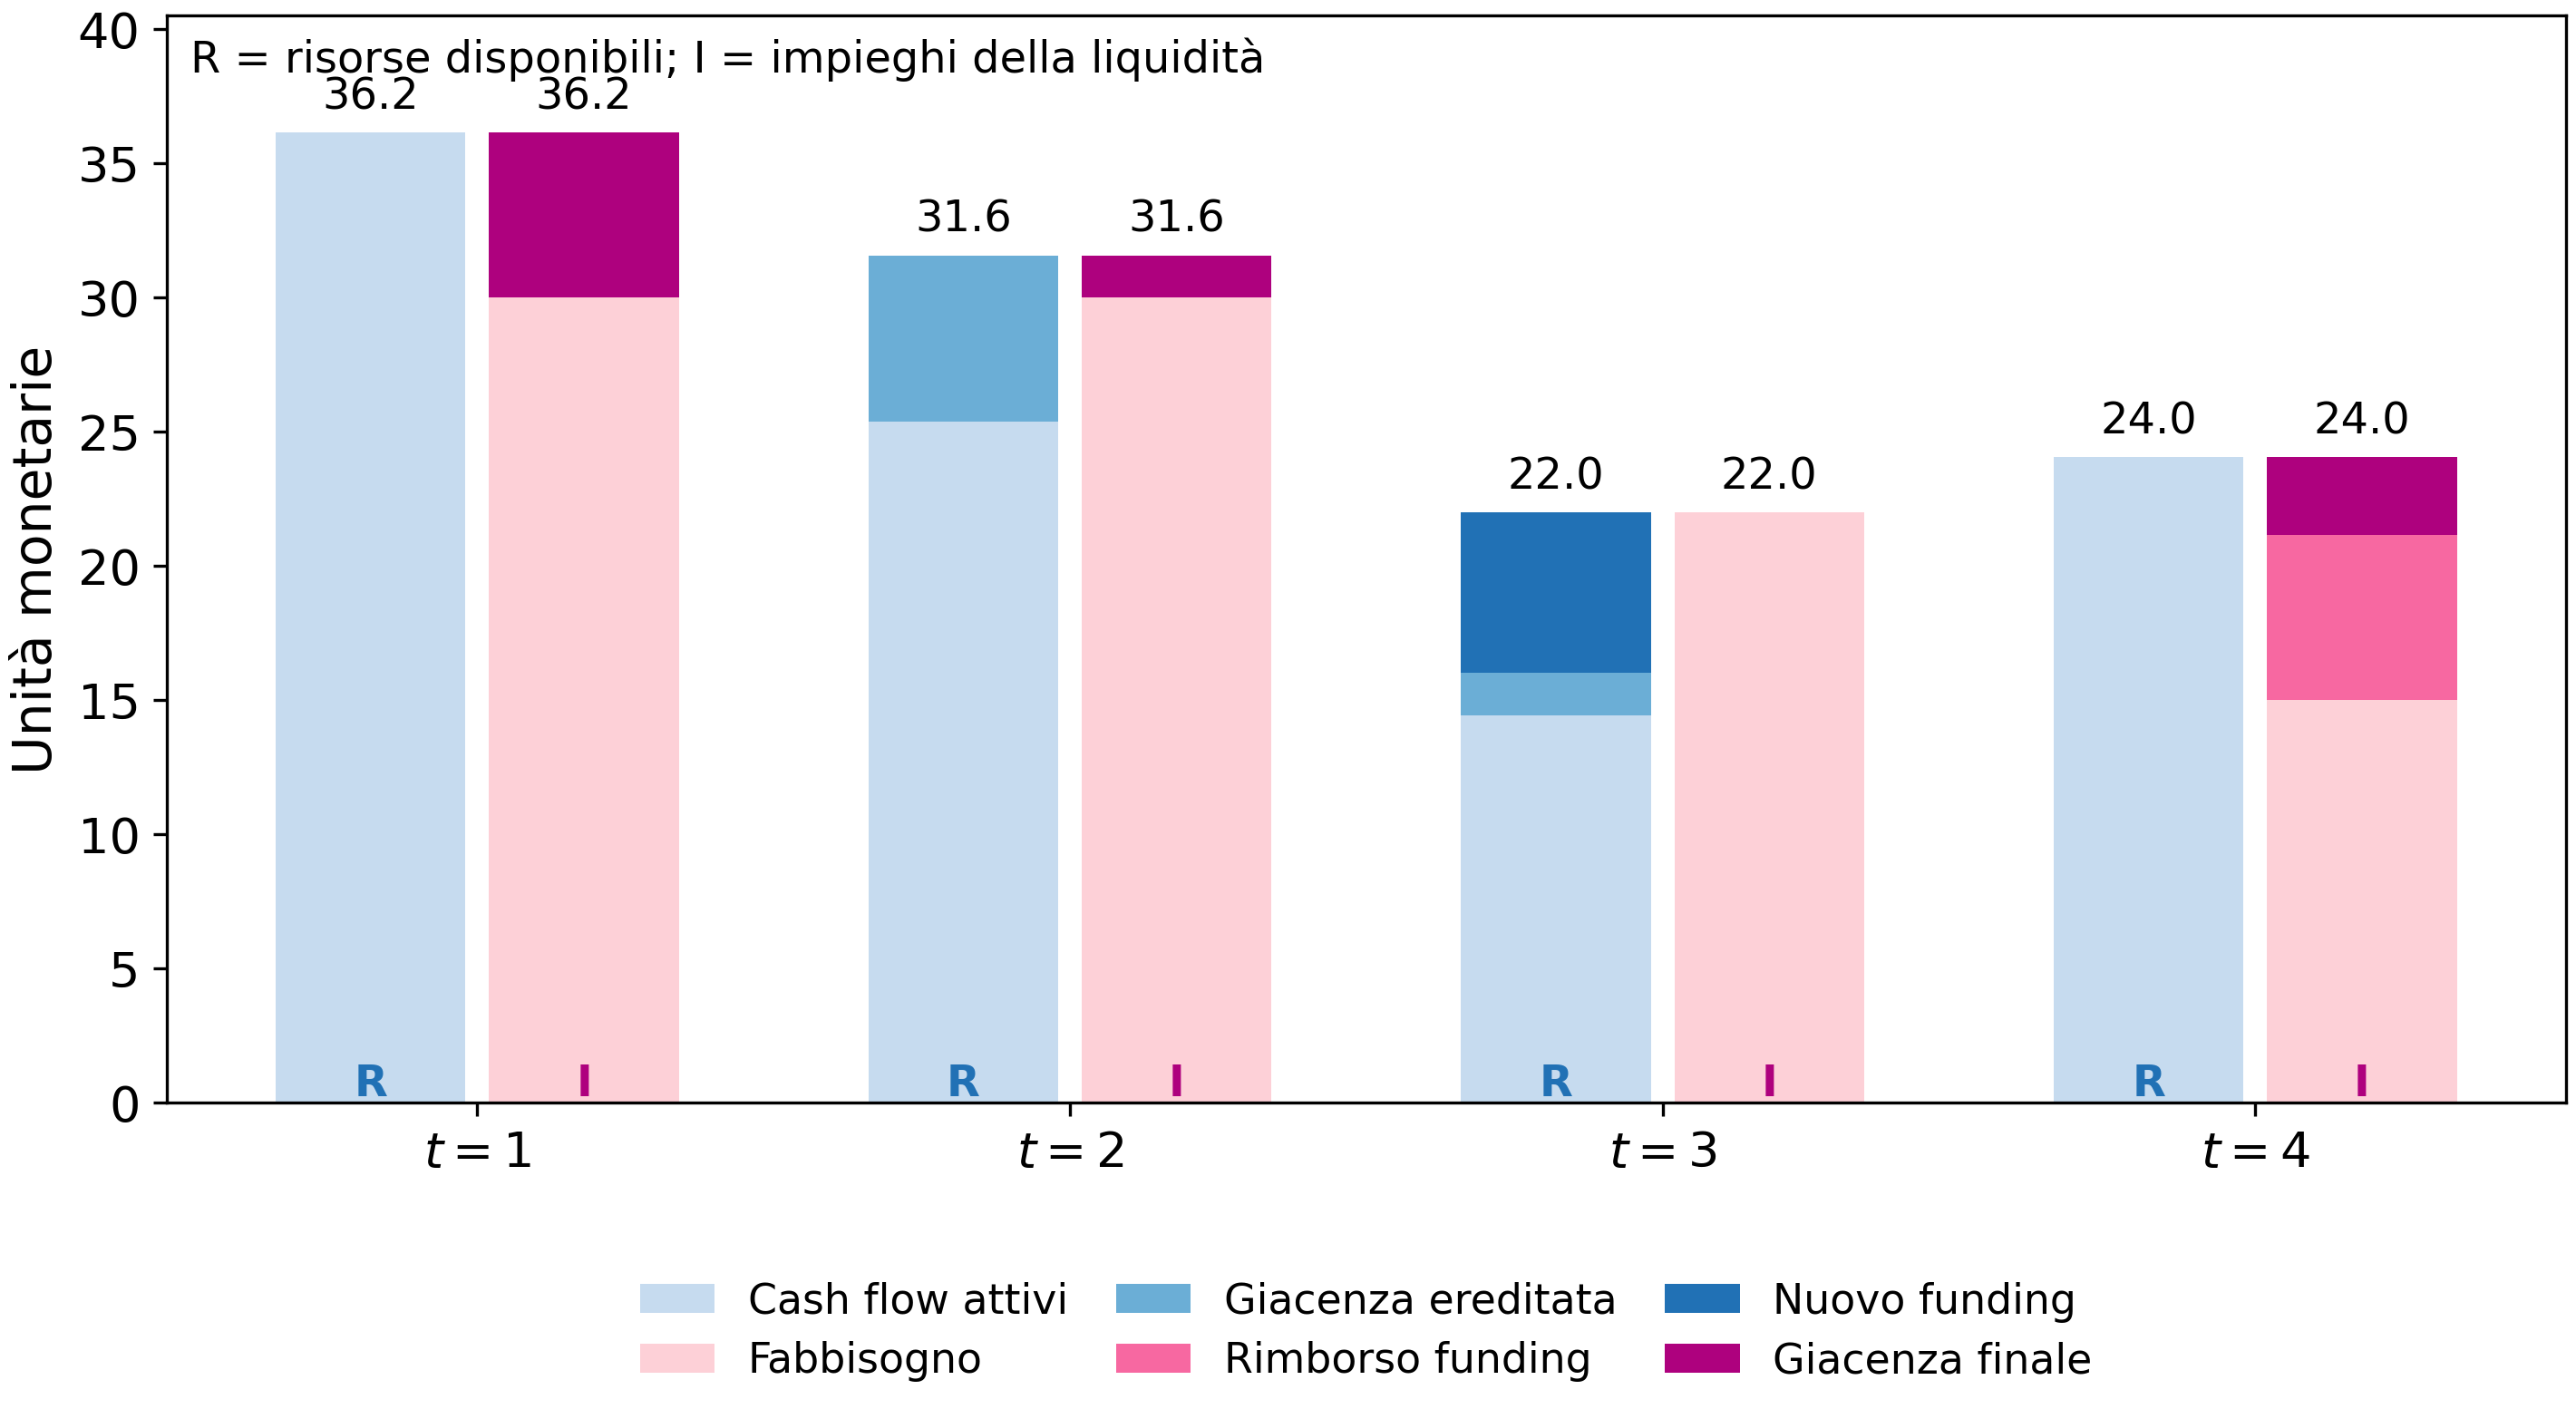
\includegraphics[width=0.94\textwidth]
{../graphics/Cap12_ALM_profili_ottimi.png}
\caption{Risorse e impieghi nelle quattro date della soluzione ottima del
caso SVB multiperiodale. La liquidit\`a accumulata trasferisce risorse verso
le date successive, mentre alla data $t=3$ il modello utilizza interamente
la capacit\`a di funding disponibile.}
\label{fig:cap12-alm-profili-ottimi}
\end{figure}

Infine, il contributo della composizione dell'attivo \`e

\[
c'x^*
\approx
3.7020,
\]

gli interessi sulle giacenze sono

\[
\sum_{t=1}^{3}r_tg_t^*
\approx
0.0402,
\]

e il costo del funding \`e

\[
\sum_{t=1}^{3}\rho_tu_t^*
=
0.1500.
\]

Pertanto,

\[
\Pi^*
\approx
3.5922.
\]

Il confronto diretto tra questo valore e il valore ottimo del problema
statico,

\[
z^{\mathrm{stat}}
\approx
3.765,
\]

non sarebbe tuttavia del tutto corretto, poich\'e la funzione obiettivo ALM
contiene anche interessi sulle giacenze e costi di funding. Per isolare
l'effetto sulla sola composizione dell'attivo \`e pi\`u informativo confrontare

\[
c'x^{\mathrm{stat}}
\approx
3.765
\]

con

\[
c'x^*
\approx
3.702.
\]

I vincoli prudenziali non risultano determinanti nella nuova soluzione:

\[
\ell'x^*
\approx
4.885
<
7,
\qquad
x_3^*=0<30.
\]

Al contrario, il limite

\[
u_3\leq6
\]

\`e raggiunto.

La sola osservazione dei vincoli attivi indica dove si concentra la scarsit\`a,
ma non ne misura ancora il valore economico. La domanda naturale diventa
quindi quale sia il valore marginale di una unit\`a aggiuntiva di risorse
disponibili nelle diverse date. Questo problema conduce direttamente
all'interpretazione duale dei bilanci temporali.

\section{Dualit\`a nell'ALM: il valore della liquidit\`a nelle diverse date}

\label{sec:cap12-dualita-alm}

Il Capitolo~\ref{cap:programmazione-lineare} ha mostrato che una variabile
duale consente di attribuire un valore marginale a una risorsa o a un
requisito del problema primale. Nel modello statico, un unico prezzo ombra
era associato al requisito aggregato di liquidit\`a.

Nel modello ALM la liquidit\`a non \`e invece concentrata in un solo vincolo.
Esiste un bilancio monetario per ciascuna data:

\[
a_t'x
+
(1+r_{t-1})g_{t-1}
+
u_t
-
(1+\rho_{t-1})u_{t-1}
-
g_t
=
d_t,
\]

con le opportune modifiche alla prima e all'ultima data.

La dualit\`a permette quindi di passare da un unico valore della liquidit\`a
a un profilo temporale di valori marginali.

\subsection{Il valore marginale dei bilanci temporali}

Associamo al bilancio della data $t$ una variabile duale

\[
\lambda_t\in\mathbb{R}.
\]

Poich\'e il vincolo di bilancio \`e un'uguaglianza, $\lambda_t$ non \`e
soggetta a un vincolo di segno.

Scrivendo il bilancio nella forma

\[
\text{risorse nette alla data }t=d_t,
\]

la convenzione adottata implica

\[
\frac{\partial\Pi^*}{\partial d_t}
=
-\lambda_t^*.
\]

Per una piccola variazione $\Delta d_t$ si ha quindi

\[
\Delta\Pi^*
\approx
-\lambda_t^*\,\Delta d_t.
\]

Se

\[
\lambda_t^*>0,
\]

un aumento unitario del fabbisogno alla data $t$ riduce localmente il
risultato ottimo di $\lambda_t^*$.

Equivalentemente, $\lambda_t^*$ misura il valore marginale di una unit\`a
aggiuntiva di liquidit\`a disponibile in quella stessa data.

Il passaggio rispetto al modello statico \`e quindi

\[
\boxed{
\text{un prezzo della liquidit\`a}
\quad\longrightarrow\quad
\text{un prezzo della liquidit\`a per ciascuna data}.
}
\]

\subsection{I valori duali nel caso SVB multiperiodale}

Per la soluzione della Sezione~\ref{sec:cap12-caso-svb-multiperiodale}, i
valori marginali dei quattro bilanci sono

\[
\lambda^*
\approx
\begin{pmatrix}
0.04524\\
0.04004\\
0.03383\\
0
\end{pmatrix}.
\]

La relazione tra posizione primale e valore marginale pu\`o essere riassunta
come segue:

\[
\begin{array}{c|c|c|c}
\hline
t & g_t^* & u_t^* & \lambda_t^*\\
\hline
1 & 6.152 & 0 & 0.04524\\
2 & 1.567 & 0 & 0.04004\\
3 & 0     & 6 & 0.03383\\
4 & 2.890 & - & 0\\
\hline
\end{array}
\]

Alla prima data, per esempio,

\[
\lambda_1^*
\approx
0.04524
\]

significa che un aumento marginale di una unit\`a del fabbisogno $d_1$
riduce il risultato ottimo di circa

\[
0.04524.
\]

Alla seconda e alla terza data il costo marginale rimane positivo, ma
diminuisce rispettivamente a

\[
0.04004
\]

e

\[
0.03383.
\]

Il risultato alla data finale richiede invece un'interpretazione specifica.

Poich\'e

\[
g_4^*
\approx
2.890>0
\]

e la giacenza terminale non riceve un valore nella funzione obiettivo, un
piccolo aumento di $d_4$ pu\`o essere assorbito semplicemente riducendo
$g_4$.

Localmente,

\[
\lambda_4^*=0.
\]

Questo non significa che la liquidit\`a alla data finale non abbia valore in
generale. Il risultato dipende dalla specificazione terminale del modello e
rimane valido finch\'e il margine rappresentato da $g_4^*$ non viene
esaurito.

\begin{figure}[htbp]
\centering
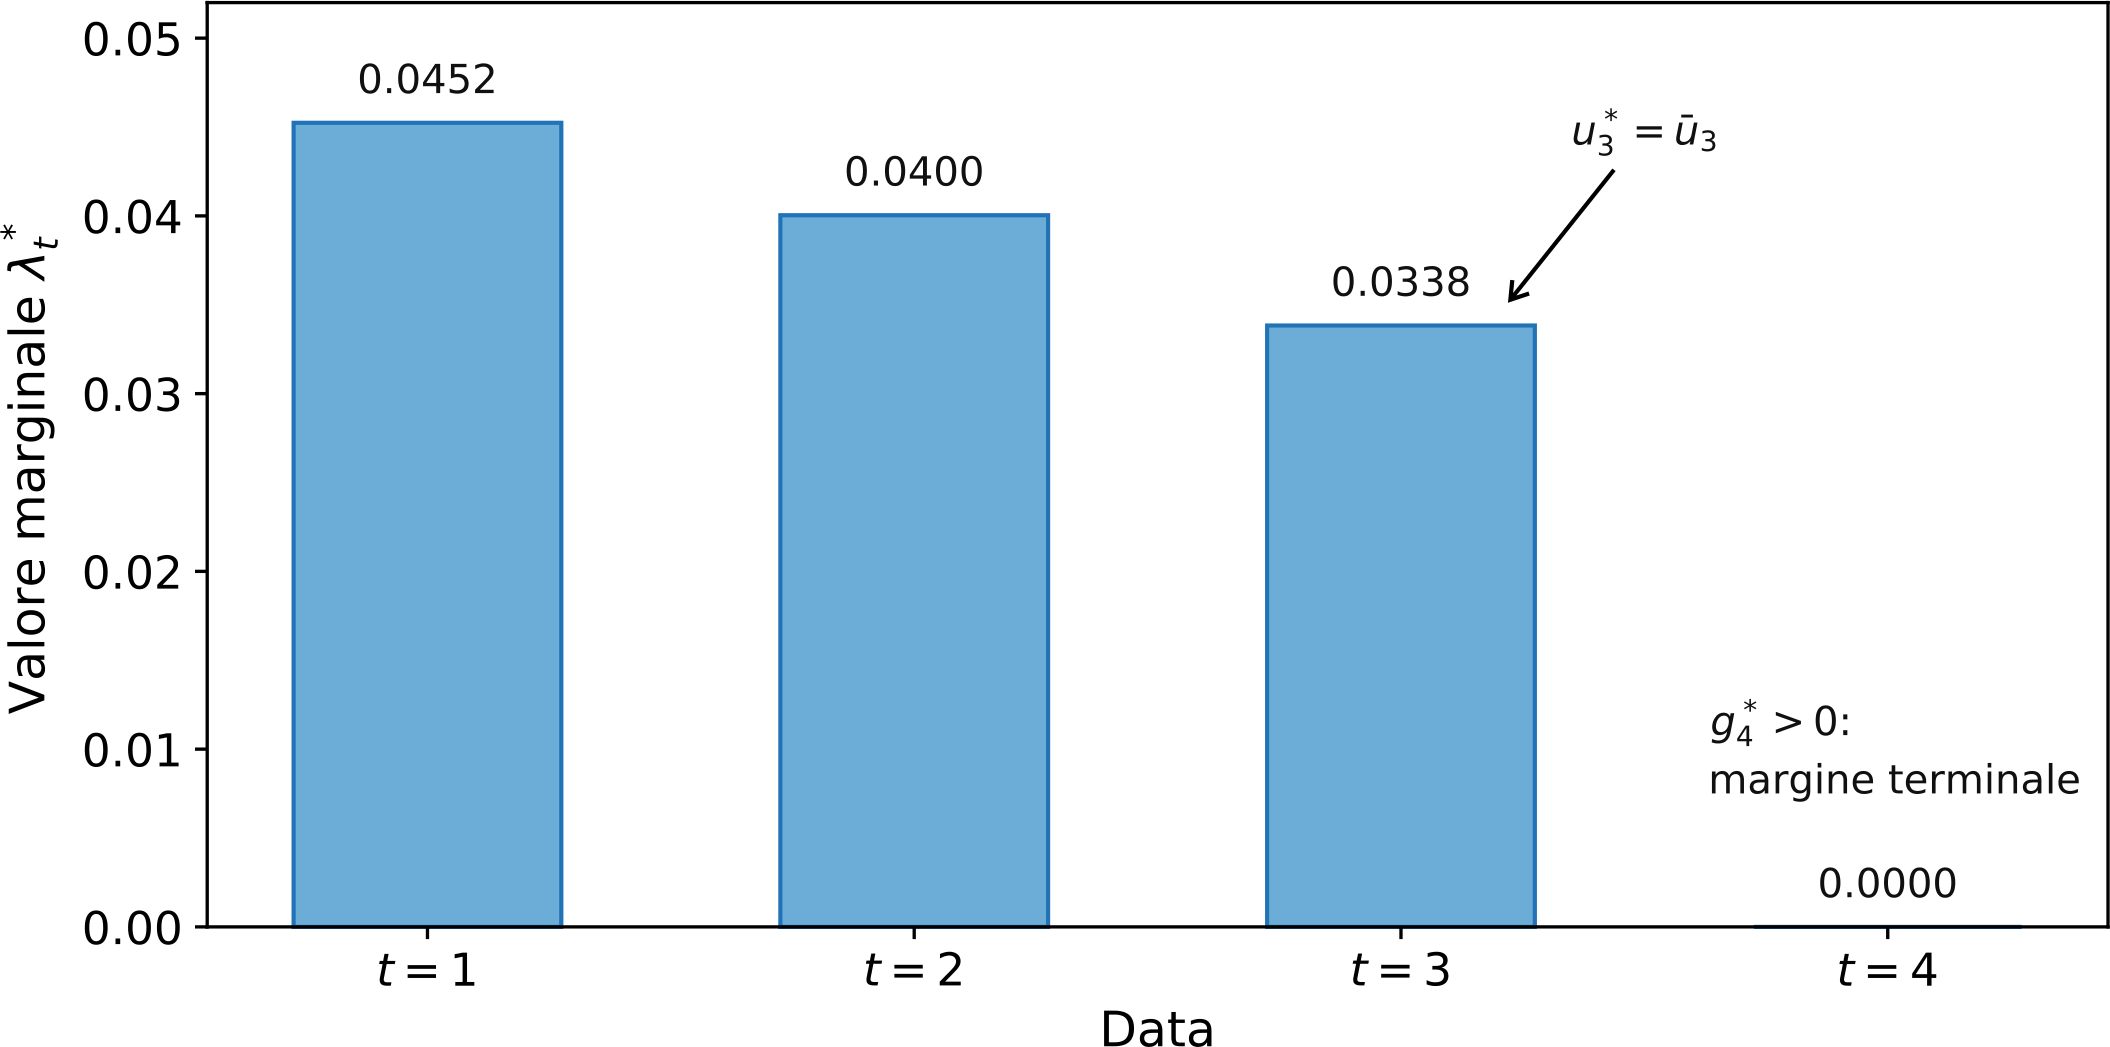
\includegraphics[width=0.88\textwidth]
{../graphics/Cap12_prezzi_ombra_scadenze.png}
\caption{Valore marginale della liquidit\`a nelle quattro date del caso SVB
multiperiodale. Il valore terminale \`e nullo localmente perch\'e la
soluzione presenta una giacenza finale positiva; alla data $t=3$ la banca
utilizza invece interamente la capacit\`a di funding disponibile.}
\label{fig:cap12-prezzi-ombra-scadenze}
\end{figure}

La Figura~\ref{fig:cap12-prezzi-ombra-scadenze} mostra un profilo decrescente
dei valori marginali. Tale andamento appartiene alla soluzione considerata e
non costituisce una propriet\`a generale dei modelli ALM: dipende dai cash
flow, dai fabbisogni, dai tassi, dai limiti di funding e dalla condizione
terminale.

\subsection{Il valore della capacit\`a di funding}

Un secondo valore duale rilevante riguarda il limite

\[
u_t\leq\bar u_t.
\]

Indichiamo con

\[
\lambda_{u,t}^*
\]

il valore marginale associato alla capacit\`a massima di funding. Localmente,

\[
\Delta\Pi^*
\approx
\lambda_{u,t}^*\,\Delta\bar u_t.
\]

Nella soluzione considerata,

\[
u_1^*<\bar u_1,
\qquad
u_2^*<\bar u_2,
\]

e i corrispondenti valori marginali sono nulli.

Alla terza data vale invece

\[
u_3^*
=
\bar u_3
=
6,
\]

e il valore duale associato al limite risulta

\[
\lambda_{u,3}^*
\approx
0.00883.
\]

Una piccola espansione della capacit\`a di funding disponibile alla data $3$
aumenterebbe quindi il valore ottimo di circa $0.00883$ per ogni unit\`a
aggiuntiva di capacit\`a.

Il risultato completa l'informazione fornita dalla soluzione primale:
l'uguaglianza

\[
u_3^*=\bar u_3
\]

individua una risorsa completamente utilizzata, mentre il corrispondente
valore duale misura quanto sarebbe economicamente utile, localmente,
allentarne il limite.

\section{Limiti del modello e passaggio all'incertezza}

\label{sec:cap12-limiti-incertezza}

Il modello sviluppato nelle sezioni precedenti permette di coordinare
composizione dell'attivo, liquidit\`a e funding lungo pi\`u date. La sua
struttura temporale \`e quindi pi\`u ricca di quella del problema statico del
Capitolo 11.

Rimane tuttavia un'ipotesi particolarmente forte: al tempo $0$ la banca
conosce l'intera traiettoria dei coefficienti che determineranno il problema
nelle date future.

\subsection{Che cosa significa deterministico}

Nel modello del capitolo sono noti al tempo $0$, tra gli altri,

\[
A^{\mathrm{CF}},
\qquad
d_t,
\qquad
r_t,
\qquad
\rho_t,
\qquad
\bar u_t.
\]

L'ipotesi deterministica non richiede che tali coefficienti siano costanti
nel tempo. Nel caso SVB multiperiodale, per esempio,

\[
r_1\neq r_2\neq r_3
\]

e anche la capacit\`a di funding varia:

\[
\bar u_1>\bar u_2>\bar u_3.
\]

Ci\`o che caratterizza il modello come deterministico \`e invece il fatto che
l'intero percorso

\[
\left\{
A^{\mathrm{CF}},
d_t,
r_t,
\rho_t,
\bar u_t
\right\}_{t=1}^{T}
\]

sia considerato noto quando il problema viene risolto.

Di conseguenza, la banca pu\`o determinare fin dal tempo $0$ l'intero piano

\[
x^*,
\qquad
g_1^*,\ldots,g_T^*,
\qquad
u_1^*,\ldots,u_{T-1}^*.
\]

Il modello risponde quindi alla domanda:

\[
\boxed{
\begin{array}{c}
\text{quale sarebbe il piano ottimo se la traiettoria futura}\\
\text{dei coefficienti fosse conosciuta?}
\end{array}
}
\]

Questa rappresentazione costituisce un benchmark utile, ma non descrive
completamente il problema decisionale affrontato da una banca reale.

\subsection{Quali elementi possono diventare incerti}

Nella realt\`a, alla data iniziale la banca non conosce con certezza le
condizioni che si manifesteranno nelle date successive.

Il vettore deterministico introdotto nella
Sezione~\ref{sec:cap12-ambiente-deterministico},

\[
\bar Z_t
=
(\bar R_t,\bar C_t,\bar F_t),
\]

pu\`o essere sostituito, in una rappresentazione incerta, da uno stato
economico-finanziario

\[
Z_t
=
(R_t,C_t,F_t).
\]

La distinzione \`e sostanziale. Nel primo caso

\[
\bar Z_t
\]

\`e un valore noto al momento della formulazione; nel secondo

\[
Z_t
\]

rappresenta uno stato futuro che non \`e ancora conosciuto al tempo $0$.

L'incertezza pu\`o quindi propagarsi ai coefficienti dell'ALM. In forma
schematica,

\[
Z_t
\quad\longrightarrow\quad
r_t,\ \rho_t,\ \bar u_t,
\]

e, quando economicamente appropriato, anche ai cash flow disponibili e ai
fabbisogni.

In particolare, il fabbisogno deterministico

\[
d_t
\]

pu\`o essere sostituito da una quantit\`a futura

\[
D_t,
\]

il cui valore dipende dalle condizioni che si realizzano.

La struttura concettuale discussa nella
Sezione~\ref{sec:cap12-stato-banca} suggerisce pi\`u precisamente

\[
D_t
=
d(Z_t,h_t),
\]

dove

\[
h_t
=
h(X_t,Z_t)
\]

dipende sia dall'ambiente esterno sia dallo stato della banca.

Non renderemo qui operative queste relazioni. Esse servono a individuare il
punto nel quale l'ipotesi deterministica dovr\`a essere abbandonata.

\subsection{Dal piano unico alle decisioni contingenti}

L'effetto pi\`u importante dell'incertezza riguarda la natura stessa delle
decisioni.

Nel modello deterministico il valore futuro di

\[
u_t
\]

pu\`o essere scelto gi\`a al tempo $0$, perch\'e i fabbisogni, i costi e la
capacit\`a di funding futuri sono noti.

In presenza di incertezza questa impostazione non \`e generalmente
appropriata. Il funding da utilizzare alla data $t$ dovrebbe poter dipendere
dalle condizioni effettivamente osservate a quella data.

Si passa quindi concettualmente da

\[
u_t
=
\text{numero fissato al tempo }0
\]

a una decisione del tipo

\[
u_t
=
u_t(\text{informazione disponibile alla data }t).
\]

La composizione iniziale $x$, invece, deve essere scelta prima di conoscere
gli stati futuri. Essa deve quindi tenere conto delle conseguenze che potranno
emergere lungo pi\`u evoluzioni possibili.

Il passaggio fondamentale pu\`o essere sintetizzato come

\[
\boxed{
\begin{array}{ccc}
\text{ALM deterministico}
&
\longrightarrow
&
\text{ALM sotto incertezza}
\\[4pt]
\text{una traiettoria nota}
&&
\text{pi\`u evoluzioni possibili}
\\[4pt]
\text{un piano fissato al tempo }0
&&
\text{decisioni compatibili con l'informazione disponibile}.
\end{array}
}
\]

Anche i valori duali ottenuti nelle sezioni precedenti devono essere letti
alla luce di questa distinzione. Essi misurano valori marginali
\emph{condizionati alla traiettoria deterministica assunta}: non incorporano
da soli il rischio che tassi, fabbisogni o disponibilit\`a di funding seguano
percorsi differenti.

Il modello deterministico rimane quindi un riferimento essenziale. Permette
di isolare la struttura dei bilanci intertemporali, identificare le date nelle
quali le risorse risultano scarse e attribuire loro un valore marginale.

Il passo successivo consiste nel mantenere questa struttura temporale
abbandonando l'ipotesi di conoscenza perfetta del futuro.

\section{Esercizi svolti}

\label{sec:cap12-esercizi-svolti}

Gli esercizi seguenti consolidano tre passaggi centrali del capitolo:
la formulazione di un problema ALM, la verifica della fattibilit\`a
intertemporale e l'interpretazione dei valori duali.

\begin{exercise}[Dalla descrizione del problema alla formulazione]

\label{ex:cap12-formulazione-alm-solver}

Una banca dispone al tempo $0$ di $50$ unit\`a monetarie, che devono essere
interamente allocate tra tre classi di attivo.

La prima classe rappresenta cassa e riserve. Produce un contributo economico
pari all'1\% dell'investimento e l'intero ammontare investito diventa
disponibile come liquidit\`a alla data $1$.

La seconda classe \`e costituita da titoli a breve scadenza. Produce un
contributo economico del $2.5\%$; il $60\%$ dell'investimento iniziale diventa
disponibile alla data $1$ e il restante $40\%$ alla data $2$.

La terza classe \`e costituita da prestiti. Produce un contributo economico
del $4.5\%$; il $10\%$ dell'investimento iniziale diventa disponibile alla
data $1$, il $30\%$ alla data $2$ e il restante $60\%$ alla data $3$.

I fabbisogni di liquidit\`a alle tre date sono rispettivamente

\[
25,\qquad18,\qquad12.
\]

La liquidit\`a non utilizzata alla data $1$ pu\`o essere trasferita alla data
$2$ con un rendimento dello $0.5\%$; quella non utilizzata alla data $2$ pu\`o
essere trasferita alla data $3$ con un rendimento dello $0.6\%$.

La banca pu\`o inoltre raccogliere funding alla data $1$ fino a un massimo di
$4$ unit\`a, con costo dell'1.5\%, e alla data $2$ fino a un massimo di $3$
unit\`a, con costo del $2\%$. Il funding raccolto in una data deve essere
rimborsato alla data successiva.

In uno scenario di stress, le perdite unitarie associate alle tre classi di
attivo sono rispettivamente

\[
0,\qquad0.03,\qquad0.08,
\]

e la perdita complessiva non pu\`o superare $2.6$.

Infine, l'investimento nei prestiti non pu\`o superare $25$ unit\`a.

A partire esclusivamente da queste informazioni:

\begin{enumerate}

\item individuare le variabili decisionali;

\item costruire i vettori e la matrice dei parametri necessari;

\item formulare matematicamente la funzione obiettivo;

\item scrivere il vincolo sulle risorse iniziali, i tre bilanci di liquidit\`a,
i vincoli prudenziali, i limiti sul funding e le condizioni di non negativit\`a;

\item raccogliere tutte le variabili in un unico vettore $z$ e scrivere il
problema nella forma matriciale necessaria per l'utilizzo di un solver LP:

\[
\min\;\widetilde c'z,
\qquad
A_{\mathrm{ub}}z\leq b_{\mathrm{ub}},
\qquad
A_{\mathrm{eq}}z=b_{\mathrm{eq}},
\]

specificando inoltre i bounds delle variabili.
\end{enumerate}

\end{exercise}

\noindent
\textbf{Soluzione.}

\begin{enumerate}

\item \textbf{Variabili decisionali.}

Indichiamo con

\[
x_1,\qquad x_2,\qquad x_3
\]

gli importi investiti al tempo $0$ rispettivamente in cassa e riserve,
titoli a breve scadenza e prestiti.

Le giacenze di liquidit\`a residue alle tre date sono

\[
g_1,\qquad g_2,\qquad g_3,
\]

mentre il funding raccolto alle prime due date \`e rappresentato da

\[
u_1,\qquad u_2.
\]

Non viene introdotto nuovo funding alla data finale, poich\'e il relativo
rimborso cadrebbe oltre l'orizzonte del modello.

Tutte le variabili sono non negative:

\[
x_j\geq0,
\qquad
j=1,2,3,
\]

\[
g_t\geq0,
\qquad
t=1,2,3,
\]

\[
u_t\geq0,
\qquad
t=1,2.
\]


\item \textbf{Costruzione dei parametri.}

Dalla descrizione delle tre classi di attivo si ricava il vettore dei
contributi economici unitari

\[
c
=
\begin{pmatrix}
0.010\\
0.025\\
0.045
\end{pmatrix}.
\]

I profili temporali con cui le risorse investite nelle tre classi diventano
disponibili determinano la matrice dei cash flow

\[
A^{\mathrm{CF}}
=
\begin{pmatrix}
1.00 & 0.60 & 0.10\\
0    & 0.40 & 0.30\\
0    & 0    & 0.60
\end{pmatrix}.
\]

Il vettore dei fabbisogni \`e

\[
d
=
\begin{pmatrix}
25\\
18\\
12
\end{pmatrix}.
\]

I rendimenti delle giacenze sono

\[
r_1=0.005,
\qquad
r_2=0.006,
\]

mentre i costi del funding sono

\[
\rho_1=0.015,
\qquad
\rho_2=0.020.
\]

La capacit\`a massima di funding \`e

\[
\bar u_1=4,
\qquad
\bar u_2=3.
\]

Il vettore delle perdite unitarie nello scenario di stress \`e

\[
\ell
=
\begin{pmatrix}
0\\
0.03\\
0.08
\end{pmatrix},
\]

con limite complessivo

\[
K=2.6.
\]

Infine, il limite di concentrazione sui prestiti \`e

\[
x_3\leq25.
\]


\item \textbf{Funzione obiettivo.}

In forma simbolica, per un orizzonte con $T=3$ date future, la funzione
obiettivo \`e

\[
\max\;
\Pi(x,g,u)
=
c'x
+
\sum_{t=1}^{2}r_tg_t
-
\sum_{t=1}^{2}\rho_tu_t.
\]

Sostituendo i valori numerici si ottiene

\[
\boxed{
\max\;
0.010x_1
+
0.025x_2
+
0.045x_3
+
0.005g_1
+
0.006g_2
-
0.015u_1
-
0.020u_2.
}
\]


\item \textbf{Vincoli del modello ALM.}

Le risorse iniziali devono essere interamente allocate:

\[
x_1+x_2+x_3=50.
\]

Alla prima data sono disponibili i cash flow prodotti dagli attivi e il
funding eventualmente raccolto in $t=1$. Il bilancio di liquidit\`a \`e

\[
x_1
+
0.60x_2
+
0.10x_3
+
u_1
=
25+g_1,
\]

ovvero

\[
x_1
+
0.60x_2
+
0.10x_3
+
u_1
-
g_1
=
25.
\]

Alla seconda data diventano disponibili i nuovi cash flow degli attivi, la
giacenza precedente capitalizzata e il nuovo funding. Deve inoltre essere
rimborsato il funding raccolto alla prima data:

\[
0.40x_2
+
0.30x_3
+
1.005g_1
+
u_2
=
18
+
1.015u_1
+
g_2.
\]

Pertanto,

\[
0.40x_2
+
0.30x_3
+
1.005g_1
+
u_2
-
1.015u_1
-
g_2
=
18.
\]

Alla data finale non viene raccolto nuovo funding:

\[
0.60x_3
+
1.006g_2
=
12
+
1.020u_2
+
g_3,
\]

ossia

\[
0.60x_3
+
1.006g_2
-
1.020u_2
-
g_3
=
12.
\]

Il vincolo sulla perdita nello scenario di stress \`e

\[
0.03x_2+0.08x_3\leq2.6.
\]

Il limite di concentrazione sui prestiti \`e

\[
x_3\leq25.
\]

I limiti sul funding sono

\[
0\leq u_1\leq4,
\qquad
0\leq u_2\leq3.
\]

Infine,

\[
x_1,x_2,x_3\geq0,
\qquad
g_1,g_2,g_3\geq0.
\]

Il programma lineare completo \`e quindi

\[
\begin{array}{ll}

\max
&
\displaystyle
0.010x_1
+
0.025x_2
+
0.045x_3
\\
& +
0.005g_1
+
0.006g_2
-
0.015u_1
-
0.020u_2
\\[8pt]

\mbox{soggetto a}
&
x_1+x_2+x_3=50,
\\[6pt]

&
x_1+0.60x_2+0.10x_3+u_1-g_1=25,
\\[6pt]

&
0.40x_2+0.30x_3+1.005g_1
+u_2-1.015u_1-g_2=18,
\\[6pt]

&
0.60x_3+1.006g_2-1.020u_2-g_3=12,
\\[6pt]

&
0.03x_2+0.08x_3\leq2.6,
\\[6pt]

&
x_3\leq25,
\\[6pt]

&
0\leq u_1\leq4,
\qquad
0\leq u_2\leq3,
\\[6pt]

&
x_1,x_2,x_3,g_1,g_2,g_3\geq0.
\end{array}
\]


\item \textbf{Forma matriciale per il solver.}

Raccogliamo le variabili secondo l'ordine

\[
z
=
\begin{pmatrix}
x_1&
x_2&
x_3&
g_1&
g_2&
g_3&
u_1&
u_2
\end{pmatrix}'.
\]

Rispetto a questo ordinamento, il vettore dei coefficienti della funzione
obiettivo in massimizzazione \`e

\[
c^{\mathrm{ALM}}
=
\begin{pmatrix}
0.010\\
0.025\\
0.045\\
0.005\\
0.006\\
0\\
-0.015\\
-0.020
\end{pmatrix}.
\]

Poich\'e il solver \texttt{scipy.optimize.linprog} utilizza una formulazione
in minimizzazione, si pone

\[
\widetilde c
=
-c^{\mathrm{ALM}},
\]

e quindi

\[
\widetilde c
=
\begin{pmatrix}
-0.010\\
-0.025\\
-0.045\\
-0.005\\
-0.006\\
0\\
0.015\\
0.020
\end{pmatrix}.
\]

Il problema passato al solver ha pertanto funzione obiettivo

\[
\min\;\widetilde c'z.
\]

Il vincolo sulle risorse iniziali e i tre bilanci temporali sono uguaglianze.
Essi possono essere raccolti nella matrice

\[
A_{\mathrm{eq}}
=
\begin{pmatrix}
1 & 1    & 1    & 0     & 0     & 0  & 0      & 0\\
1 & 0.60 & 0.10 & -1    & 0     & 0  & 1      & 0\\
0 & 0.40 & 0.30 & 1.005 & -1    & 0  & -1.015 & 1\\
0 & 0    & 0.60 & 0     & 1.006 & -1 & 0      & -1.020
\end{pmatrix},
\]

con

\[
b_{\mathrm{eq}}
=
\begin{pmatrix}
50\\
25\\
18\\
12
\end{pmatrix}.
\]

I due vincoli espressi come disuguaglianze sono

\[
0.03x_2+0.08x_3\leq2.6
\]

e

\[
x_3\leq25.
\]

Pertanto,

\[
A_{\mathrm{ub}}
=
\begin{pmatrix}
0 & 0.03 & 0.08 & 0 & 0 & 0 & 0 & 0\\
0 & 0    & 1    & 0 & 0 & 0 & 0 & 0
\end{pmatrix},
\]

e

\[
b_{\mathrm{ub}}
=
\begin{pmatrix}
2.6\\
25
\end{pmatrix}.
\]

Infine, i limiti delle variabili sono

\[
\begin{array}{c|c}
\text{variabili} & \text{bounds}\\
\hline
x_1,x_2,x_3 & [0,+\infty)\\
g_1,g_2,g_3 & [0,+\infty)\\
u_1 & [0,4]\\
u_2 & [0,3].
\end{array}
\]

La formulazione da trasmettere al solver \`e quindi completamente
specificata da

\[
\boxed{
\begin{array}{c}
\displaystyle
\min\;\widetilde c'z
\\[6pt]
A_{\mathrm{eq}}z=b_{\mathrm{eq}},
\\[4pt]
A_{\mathrm{ub}}z\leq b_{\mathrm{ub}},
\\[4pt]
\underline z\leq z\leq\overline z.
\end{array}
}
\]

Il passaggio decisivo non consiste nell'applicazione del solver, ma nella
traduzione coerente della descrizione finanziaria in variabili, coefficienti
e vincoli. Una volta costruita correttamente questa rappresentazione, il
problema \`e un programma lineare standard e pu\`o essere risolto
numericamente senza ulteriori modifiche alla sua struttura economica.

\end{enumerate}


\begin{exercise}[Fattibilit\`a temporale e limite al funding]

\label{ex:cap12-fattibilita-funding}

Una banca ha investito al tempo $0$ in due classi di attivo secondo la
composizione

\[
x=
\begin{pmatrix}
20\\
20
\end{pmatrix}.
\]

La distribuzione temporale dei cash flow prodotti dagli attivi \`e descritta
dalla matrice

\[
A^{\mathrm{CF}}
=
\begin{pmatrix}
0.70 & 0.10\\
0.30 & 0.30\\
0    & 0.60
\end{pmatrix}.
\]

I fabbisogni di liquidit\`a alle tre date sono

\[
d'
=
(15,\;14,\;8).
\]

La liquidit\`a residua alla prima data pu\`o essere trasferita alla seconda
con rendimento

\[
r_1=0.005.
\]

Si assume che non venga raccolto funding alla prima data,

\[
u_1=0,
\]

mentre alla seconda data la banca pu\`o ricorrere a funding che dovr\`a essere
rimborsato alla data finale con costo

\[
\rho_2=0.020.
\]

In condizioni ordinarie la capacit\`a di funding alla seconda data \`e

\[
\bar u_2=3.
\]

\begin{enumerate}

\item Calcolare il profilo temporale dei cash flow prodotto dagli attivi.

\item Verificare se la composizione assegnata permette di soddisfare i
fabbisogni alle tre date senza ricorrere al funding.

\item Determinare il funding minimo necessario alla seconda data e calcolare
la giacenza terminale risultante.

\item Supporre ora che la capacit\`a massima di funding alla seconda data si
riduca a

\[
\bar u_2=0.8.
\]

Stabilire se il piano rimane ammissibile e interpretare il risultato.

\end{enumerate}

\end{exercise}

\noindent
\textbf{Soluzione.}

\begin{enumerate}

\item Il profilo dei cash flow \`e

\[
A^{\mathrm{CF}}x
=
\begin{pmatrix}
0.70 & 0.10\\
0.30 & 0.30\\
0    & 0.60
\end{pmatrix}
\begin{pmatrix}
20\\
20
\end{pmatrix}
=
\begin{pmatrix}
16\\
12\\
12
\end{pmatrix}.
\]

\item Alla prima data, ponendo $u_1=0$,

\[
16=15+g_1,
\]

da cui

\[
g_1=1.
\]

Alla seconda data, in assenza di funding, le risorse disponibili sarebbero

\[
12+1.005(1)
=
13.005.
\]

Il fabbisogno \`e invece

\[
d_2=14.
\]

Pertanto

\[
13.005<14
\]

e la composizione non \`e temporalmente fattibile senza funding.

Il punto importante \`e che l'insufficienza emerge alla seconda data:
non pu\`o essere compensata utilizzando anticipatamente il cash flow pari a
$12$ che sar\`a disponibile soltanto alla data successiva.

\item Ponendo $g_2=0$, il bilancio della seconda data richiede

\[
12
+
1.005(1)
+
u_2
=
14.
\]

Il funding minimo \`e quindi

\[
u_2
=
14-13.005
=
0.995.
\]

Alla data finale il rimborso dovuto \`e

\[
1.020(0.995)
=
1.0149.
\]

Il bilancio terminale diventa

\[
12
=
8
+
1.0149
+
g_3,
\]

da cui

\[
g_3
=
2.9851.
\]

Il funding anticipa quindi $0.995$ unit\`a alla seconda data e genera alla
terza un rimborso pari a $1.0149$.

\item Se

\[
\bar u_2=0.8,
\]

il funding massimo disponibile sarebbe inferiore al fabbisogno minimo

\[
u_2^{\min}=0.995.
\]

La composizione considerata diventerebbe quindi non ammissibile:

\[
\bar u_2<u_2^{\min}.
\]

\end{enumerate}

L'esercizio distingue due concetti che non devono essere confusi:
l'esistenza di risorse lungo l'intero orizzonte e la loro disponibilit\`a
nella data nella quale devono essere utilizzate.


\begin{exercise}[Interpretazione dei valori duali]

\label{ex:cap12-valori-duali}

Nel caso SVB multiperiodale della
Sezione~\ref{sec:cap12-caso-svb-multiperiodale}, i valori marginali associati
ai quattro bilanci temporali sono

\[
\lambda^*
\approx
\begin{pmatrix}
0.04524\\
0.04004\\
0.03383\\
0
\end{pmatrix}.
\]

Il valore duale associato al limite

\[
u_3\leq\bar u_3
\]

\`e inoltre

\[
\lambda_{u,3}^*
\approx
0.00883.
\]

Si assuma che le variazioni considerate siano sufficientemente piccole da
non modificare la struttura della soluzione ottima.

\begin{enumerate}

\item Stimare l'effetto sul valore ottimo di un aumento

\[
\Delta d_2=0.5.
\]

\item Interpretare il risultato

\[
\lambda_4^*=0
\]

sapendo che

\[
g_4^*\approx2.890.
\]

\item Stimare l'effetto di un aumento unitario della capacit\`a di funding
alla terza data.

\item Spiegare perch\'e queste valutazioni devono essere interpretate
localmente.

\end{enumerate}

\end{exercise}

\noindent
\textbf{Soluzione.}

\begin{enumerate}

\item Per una piccola variazione del fabbisogno vale

\[
\Delta\Pi^*
\approx
-\lambda_2^*\,\Delta d_2.
\]

Pertanto

\[
\Delta\Pi^*
\approx
-0.04004(0.5)
=
-0.02002.
\]

Un aumento di mezzo punto del fabbisogno alla seconda data riduce quindi
localmente il valore ottimo di circa $0.020$.

\item Il risultato

\[
\lambda_4^*=0
\]

non significa che la liquidit\`a alla data finale sia priva di significato
finanziario.

Nella soluzione considerata esiste infatti una giacenza terminale positiva:

\[
g_4^*\approx2.890.
\]

Un piccolo aumento di $d_4$ pu\`o essere assorbito riducendo questa giacenza,
senza richiedere una modifica della composizione dell'attivo o del piano di
funding e senza modificare localmente la funzione obiettivo.

Il valore marginale nullo riflette quindi l'esistenza di un margine terminale
nella soluzione considerata.

\item Per il limite sulla capacit\`a di funding vale localmente

\[
\Delta\Pi^*
\approx
\lambda_{u,3}^*
\Delta\bar u_3.
\]

Con

\[
\Delta\bar u_3=1
\]

si ottiene

\[
\Delta\Pi^*
\approx
0.00883.
\]

Una unit\`a aggiuntiva di capacit\`a di funding alla terza data aumenterebbe
quindi il risultato massimo di circa $0.00883$.

\item I valori duali descrivono la pendenza locale della funzione valore
rispetto ai termini noti o ai limiti considerati.

Se una variazione sufficientemente ampia modifica i vincoli determinanti
della soluzione, anche i corrispondenti valori marginali possono cambiare.
Non \`e quindi corretto utilizzare indefinitamente lo stesso prezzo ombra
per variazioni arbitrarie dei parametri.

\end{enumerate}

Il confronto tra soluzione primale e valori duali mette in evidenza due
informazioni complementari: il primale mostra come vengono impiegate le
risorse disponibili, mentre il duale quantifica il valore marginale di una
variazione dei requisiti o delle risorse scarse.

\section{Esercizi proposti}

\label{sec:cap12-esercizi-proposti}


\begin{exercise}[Cash flow aggregati e distribuzione temporale]

\label{ex:cap12-proposto-cashflow-temporali}

Una banca considera tre classi di attivo. La matrice dei cash flow \`e

\[
A^{\mathrm{CF}}
=
\begin{pmatrix}
0.80 & 0.30 & 0.10\\
0.20 & 0.40 & 0.30\\
0    & 0.30 & 0.60
\end{pmatrix},
\]

e la composizione iniziale \`e

\[
x'
=
(10,\;20,\;30).
\]

I fabbisogni sono

\[
d'
=
(16,\;21,\;18).
\]

Si assumano, per semplicit\`a,

\[
r_1=r_2=0.
\]

Alla seconda data la banca pu\`o raccogliere funding al tasso

\[
\rho_2=0.02.
\]

\begin{enumerate}

\item Calcolare il profilo temporale

\[
A^{\mathrm{CF}}x.
\]

\item Verificare che il cash flow complessivo prodotto lungo l'orizzonte
coincida con l'ammontare inizialmente investito.

\item Stabilire se i fabbisogni possono essere soddisfatti senza funding,
tenendo conto del trasferimento delle giacenze tra date consecutive.

\item Determinare il funding minimo necessario alla seconda data e la
giacenza terminale risultante.

\item Spiegare perch\'e il confronto tra

\[
\sum_t d_t
\]

e il cash flow complessivo dell'attivo non \`e sufficiente per stabilire
l'ammissibilit\`a del piano.

\end{enumerate}

\end{exercise}

\noindent
\textit{Risultati:}

\[
A^{\mathrm{CF}}x
=
\begin{pmatrix}
17\\
19\\
24
\end{pmatrix},
\qquad
\sum_{t=1}^{3}(A^{\mathrm{CF}}x)_t=60.
\]

Alla prima data

\[
g_1=1.
\]

Alla seconda data rimane un deficit pari a $1$, per cui il funding minimo
\`e

\[
u_2=1.
\]

Tenendo conto del rimborso alla data finale,

\[
g_3=24-18-1.02=4.98.
\]


\begin{exercise}[Due portafogli con diversa struttura temporale]

\label{ex:cap12-proposto-confronto-portafogli}

Si consideri la matrice

\[
A^{\mathrm{CF}}
=
\begin{pmatrix}
0.90 & 0.40 & 0.10\\
0.10 & 0.40 & 0.30\\
0    & 0.20 & 0.60
\end{pmatrix}
\]

e i due portafogli

\[
x^{(A)}
=
\begin{pmatrix}
20\\
20\\
10
\end{pmatrix},
\qquad
x^{(B)}
=
\begin{pmatrix}
10\\
20\\
20
\end{pmatrix}.
\]

Entrambi utilizzano risorse iniziali pari a

\[
A_0=50.
\]

I fabbisogni sono

\[
d'
=
(22,\;16,\;10).
\]

I parametri finanziari sono

\[
r_1=0.004,
\qquad
r_2=0.005,
\]

\[
\rho_1=0.014,
\qquad
\rho_2=0.018,
\]

con

\[
\bar u_1=5,
\qquad
\bar u_2=4.
\]

\begin{enumerate}

\item Calcolare i profili

\[
A^{\mathrm{CF}}x^{(A)}
\qquad\text{e}\qquad
A^{\mathrm{CF}}x^{(B)}.
\]

\item Verificare se il portafoglio $A$ pu\`o soddisfare i tre fabbisogni
senza ricorrere al funding.

\item Per il portafoglio $B$, determinare il funding minimo necessario alla
prima data.

\item Verificare se la capacit\`a massima di funding alla seconda data
permette di proseguire il piano.

\item Interpretare la differenza tra i due portafogli dal punto di vista
dell'ALM.

\end{enumerate}

\end{exercise}

\noindent
\textit{Risultati:}

\[
A^{\mathrm{CF}}x^{(A)}
=
\begin{pmatrix}
27\\
13\\
10
\end{pmatrix},
\qquad
A^{\mathrm{CF}}x^{(B)}
=
\begin{pmatrix}
19\\
15\\
16
\end{pmatrix}.
\]

Il portafoglio $A$ \`e finanziariamente ammissibile senza funding.

Per il portafoglio $B$ occorre alla prima data

\[
u_1=3.
\]

Alla seconda data il funding minimo richiesto \`e circa

\[
u_2=4.042,
\]

ma

\[
\bar u_2=4.
\]

Il portafoglio $B$ non \`e quindi ammissibile.


\begin{exercise}[Formulazione completa di un problema ALM]

\label{ex:cap12-proposto-formulazione-completa}

Una banca dispone di

\[
A_0=50
\]

unit\`a monetarie e pu\`o scegliere tra tre classi di attivo.

I parametri dell'attivo sono

\[
\begin{array}{c|cc}
\hline
j & c_j & \ell_j\\
\hline
1 & 0.015 & 0\\
2 & 0.030 & 0.04\\
3 & 0.045 & 0.10\\
\hline
\end{array}
\]

e

\[
A^{\mathrm{CF}}
=
\begin{pmatrix}
0.90 & 0.40 & 0.10\\
0.10 & 0.40 & 0.30\\
0    & 0.20 & 0.60
\end{pmatrix}.
\]

I parametri temporali sono

\[
\begin{array}{c|cccc}
\hline
t & d_t & r_t & \rho_t & \bar u_t\\
\hline
1 & 20 & 0.004 & 0.014 & 5\\
2 & 18 & 0.005 & 0.018 & 4\\
3 & 10 & -     & -     & -\\
\hline
\end{array}
\]

e il limite alla perdita sotto stress \`e

\[
\ell'x\leq3.2.
\]

La terza classe di attivo non pu\`o inoltre superare

\[
x_3\leq20.
\]

\begin{enumerate}

\item Individuare tutte le variabili decisionali.

\item Scrivere la funzione obiettivo prima in forma simbolica e poi in forma
numerica.

\item Scrivere il vincolo sulle risorse iniziali.

\item Scrivere i tre bilanci di liquidit\`a prima in forma simbolica e poi
sostituendo i coefficienti numerici.

\item Completare il programma lineare con i limiti di funding, il vincolo di
stress, il limite di concentrazione e le condizioni di non negativit\`a.

\item Indicare quali coefficienti del modello potrebbero dipendere
dall'ambiente economico-finanziario

\[
\bar Z_t=(\bar R_t,\bar C_t,\bar F_t).
\]

\end{enumerate}

\end{exercise}

\noindent
\textit{Risultati di controllo:} le variabili sono

\[
x_1,x_2,x_3,
\qquad
g_1,g_2,g_3,
\qquad
u_1,u_2.
\]

La funzione obiettivo numerica \`e

\[
\max\;
0.015x_1+0.030x_2+0.045x_3
+0.004g_1+0.005g_2
-0.014u_1-0.018u_2.
\]

Il primo bilancio \`e

\[
0.90x_1+0.40x_2+0.10x_3+u_1-g_1=20.
\]


\begin{exercise}[Sensitivit\`a dei fabbisogni e della capacit\`a di funding]

\label{ex:cap12-proposto-sensitivita}

Nel caso SVB multiperiodale sono stati ottenuti i valori marginali

\[
\lambda^*
\approx
\begin{pmatrix}
0.04524\\
0.04004\\
0.03383\\
0
\end{pmatrix}
\]

per i quattro bilanci temporali.

Il valore duale del limite sulla capacit\`a di funding alla terza data \`e

\[
\lambda_{u,3}^*
\approx
0.00883.
\]

Si considerino variazioni sufficientemente piccole da non modificare la
struttura della soluzione ottima.

\begin{enumerate}

\item Stimare la variazione del valore ottimo se

\[
d_1
\]

aumenta di $0.4$.

\item Ripetere il calcolo per un aumento di $0.4$ di $d_3$.

\item Stimare il beneficio di un aumento pari a $0.5$ della capacit\`a

\[
\bar u_3.
\]

\item Spiegare perch\'e un piccolo aumento di $d_4$ ha valore marginale nullo
nella soluzione considerata.

\item Stabilire se sarebbe corretto utilizzare

\[
\lambda_4^*=0
\]

per valutare un aumento di $d_4$ pari a $4$ unit\`a, sapendo che

\[
g_4^*\approx2.890.
\]

\end{enumerate}

\end{exercise}

\noindent
\textit{Risultati:}

\[
\Delta\Pi^*
\approx
-0.04524(0.4)
=
-0.01810
\]

per la prima data,

\[
\Delta\Pi^*
\approx
-0.03383(0.4)
=
-0.01353
\]

per la terza data, e

\[
\Delta\Pi^*
\approx
0.00883(0.5)
=
0.00442
\]

per l'espansione della capacit\`a di funding.

Il valore $\lambda_4^*=0$ non pu\`o essere esteso automaticamente a una
variazione di $4$ unit\`a, poich\'e essa supera la giacenza terminale
disponibile nella soluzione di riferimento.


\begin{exercise}[Dal modello deterministico all'incertezza]

\label{ex:cap12-proposto-deterministico-incertezza}

Nel modello ALM deterministico, al tempo $0$ sono considerati noti

\[
d_t,
\qquad
r_t,
\qquad
\rho_t,
\qquad
\bar u_t,
\]

per tutte le date future.

Supponiamo invece che alla data $2$ possano manifestarsi condizioni normali
oppure condizioni di stress, con differenti livelli dei fabbisogni e della
capacit\`a di funding.

\begin{enumerate}

\item Spiegare quale ipotesi del modello deterministico viene meno.

\item Indicare perch\'e non sarebbe generalmente corretto fissare al tempo
$0$ un unico valore di $u_2$ senza conoscere quale condizione si
realizzer\`a.

\item Distinguere la natura della decisione iniziale $x$ da quella della
decisione di funding alla data $2$.

\item Spiegare che cosa dovrebbe significare, in presenza di incertezza,

\[
u_2
=
u_2(\text{informazione disponibile alla data }2).
\]

\item Indicare quali elementi della struttura ALM sviluppata nel capitolo
rimangono comunque utili anche quando l'ipotesi deterministica viene
abbandonata.

\end{enumerate}

\end{exercise}

\section{Sintesi}

\label{sec:cap12-sintesi}

Il passaggio dalla programmazione lineare statica all'Asset--Liability
Management deterministico consiste soprattutto nell'introdurre
esplicitamente la dimensione temporale della liquidit\`a.

I risultati principali del capitolo possono essere riassunti nei seguenti
punti.

\begin{enumerate}

\item \textbf{La liquidit\`a aggregata non garantisce la liquidit\`a alle
diverse scadenze.}

Nel modello statico del Capitolo 11 la disponibilit\`a di liquidit\`a era
rappresentata da un unico vincolo

\[
q'x\geq Q_{\min}.
\]

In un problema ALM occorre invece verificare che le risorse monetarie siano
disponibili nelle date nelle quali devono essere utilizzate. Il vincolo
aggregato viene quindi sostituito da una successione di bilanci temporali.

\item \textbf{La matrice dei cash flow collega l'allocazione iniziale alle
risorse future.}

Se

\[
A^{\mathrm{CF}}
=
(a_{tj}),
\]

il coefficiente $a_{tj}$ descrive la quantit\`a di liquidit\`a resa disponibile
alla data $t$ da una unit\`a investita inizialmente nella classe di attivo $j$.

Il vettore

\[
A^{\mathrm{CF}}x
\]

determina quindi il profilo temporale dei cash flow generato dalla
composizione dell'attivo.

\item \textbf{Le giacenze e il funding collegano date consecutive.}

La giacenza

\[
g_t
\]

trasferisce liquidit\`a verso la data successiva e diventa

\[
(1+r_t)g_t.
\]

Il funding

\[
u_t
\]

produce invece liquidit\`a alla data corrente ma genera alla data successiva
un obbligo pari a

\[
(1+\rho_t)u_t.
\]

I due strumenti realizzano quindi collegamenti intertemporali di segno
economico opposto.

\item \textbf{Il problema ALM deterministico rimane un programma lineare.}

Le decisioni riguardano simultaneamente

\[
x_j,
\qquad
g_t,
\qquad
u_t.
\]

La funzione obiettivo considera il contributo economico dell'attivo, il
rendimento delle giacenze mantenute tra date successive e il costo del
funding:

\[
\max\;
\Pi(x,g,u)
=
\sum_{j=1}^{n}c_jx_j
+
\sum_{t=1}^{T-1}r_tg_t
-
\sum_{t=1}^{T-1}\rho_tu_t.
\]

I bilanci temporali, i limiti alla disponibilit\`a di funding e gli eventuali
vincoli prudenziali completano la formulazione.

La presenza di pi\`u date aumenta la struttura del problema, ma non modifica
la sua natura lineare.

\item \textbf{La soluzione statica pu\`o risultare inadeguata quando viene
considerato il profilo temporale dei flussi.}

Nel caso SVB multiperiodale, la soluzione ottenuta con il modello statico
soddisfa il requisito aggregato di liquidit\`a, ma non riesce a finanziare
tutti i fabbisogni alle rispettive date, neppure utilizzando completamente
la capacit\`a di funding disponibile.

La soluzione ALM modifica quindi la composizione iniziale dell'attivo per
tenere conto non soltanto della redditivit\`a e dei vincoli prudenziali, ma
anche della distribuzione temporale dei cash flow.

Nel caso considerato la terza data emerge come particolarmente critica:

\[
u_3^*=\bar u_3=6,
\]

mentre il vincolo di stress e il limite di concentrazione non risultano
determinanti per la soluzione ottima.

\item \textbf{La dualit\`a attribuisce un valore marginale alla liquidit\`a
nelle diverse date.}

A ciascun bilancio temporale pu\`o essere associato un valore duale

\[
\lambda_t^*,
\]

che misura localmente l'effetto sul valore ottimo di una variazione del
fabbisogno alla data $t$:

\[
\Delta\Pi^*
\approx
-\lambda_t^*\,\Delta d_t.
\]

Nel caso SVB i valori marginali differiscono tra le date. La liquidit\`a non
ha quindi un unico valore economico indipendente dalla scadenza.

Analogamente, il valore duale associato al limite

\[
u_t\leq\bar u_t
\]

misura il beneficio marginale di una maggiore capacit\`a di funding.

Queste interpretazioni sono locali: variazioni sufficientemente ampie dei
parametri possono modificare la struttura della soluzione ottima e quindi
anche i corrispondenti valori marginali.

\item \textbf{Il carattere deterministico riguarda la conoscenza del futuro,
non la costanza dei parametri.}

Nel modello sviluppato nel capitolo i coefficienti possono variare nel tempo,
ma la loro intera traiettoria viene considerata nota al tempo $0$.

La banca pu\`o quindi determinare fin dall'inizio il piano completo

\[
x^*,
\qquad
g_1^*,\ldots,g_T^*,
\qquad
u_1^*,\ldots,u_{T-1}^*.
\]

Questa ipotesi costituisce il principale limite del modello.

In presenza di incertezza, le condizioni economico-finanziarie future

\[
Z_t=(R_t,C_t,F_t)
\]

non sono note al tempo $0$ e alcune decisioni future devono dipendere
dall'informazione effettivamente disponibile quando vengono assunte.

\end{enumerate}

Il percorso sviluppato nel capitolo pu\`o quindi essere sintetizzato come

\[
\boxed{
\begin{array}{c}
\text{allocazione iniziale dell'attivo}
\\[3pt]
\downarrow
\\[3pt]
\text{cash flow distribuiti nel tempo}
\\[3pt]
\downarrow
\\[3pt]
\text{bilanci di liquidit\`a intertemporali}
\\[3pt]
\downarrow
\\[3pt]
\text{giacenze e funding}
\\[3pt]
\downarrow
\\[3pt]
\text{soluzione ottima e valori marginali per scadenza}.
\end{array}
}
\]

L'Asset--Liability Management deterministico fornisce cos\`i il ponte tra la
programmazione lineare statica e i problemi decisionali nei quali la
dimensione temporale e, successivamente, l'incertezza diventano componenti
essenziali del modello.